\documentclass[12pt]{beamer}
\usetheme{Malmoe}
\usepackage{siunitx}
\usepackage{hyperref}
\usepackage{cancel}
\sisetup{
  per-mode = fraction,
  fraction-function = \frac
}
\usepackage{extpfeil} %for the arrows
\usepackage{cancel} %strikethrough

\usepackage{tikz}
\usepackage{graphicx}  % To include images
\usetikzlibrary{shapes.geometric, arrows}

% Define block styles for the flowchart
\tikzstyle{process} = [rectangle, minimum width=2.4cm, minimum height=0.5cm, text centered, draw=black, fill=blue!10]
\tikzstyle{imageblock} = [rectangle, minimum width=2.4cm, minimum height=1.5cm, text centered] % New style for image node
\tikzstyle{arrow} = [thick,->,>=stealth]

\begin{document}


\title{Paper Presentation: Depth Anything}
\subtitle{\begin{itemize}
        \item Depth Anything: Unleashing the Power of Large-Scale Unlabeled Data (V1)
        \item Depth Anything V2 (V2)
    \end{itemize}}
\author{Benjamin Stadler}
\institute{Tsinghua University \\
    Machine Vision (Fall 2024) \\
Contact: \texttt{\href{mailto:bestadle@ethz.ch}{bestadle@ethz.ch}}}
\date{October 2024}


\begin{frame}
\titlepage
\end{frame}


\begin{frame}
    \frametitle{At a Glance}

    \begin{itemize}
        \item[What] Molecular Depth Estimation (MDE)
        \item[Who] HKU, TikTok
        \item[When] April 2024 (V1), June 2024 (V2)
        \item[How]
        \begin{itemize}
            \item[V1] known techniques + train with \underline{unlabeled data}
            \item[V2] technique from V1 + train with \underline{synthetic data}
        \end{itemize}
    \end{itemize}
    
    \begin{figure}
        \centering
        \includegraphics[width=0.49\textwidth]{./figures/huashan_orig.jpg}
        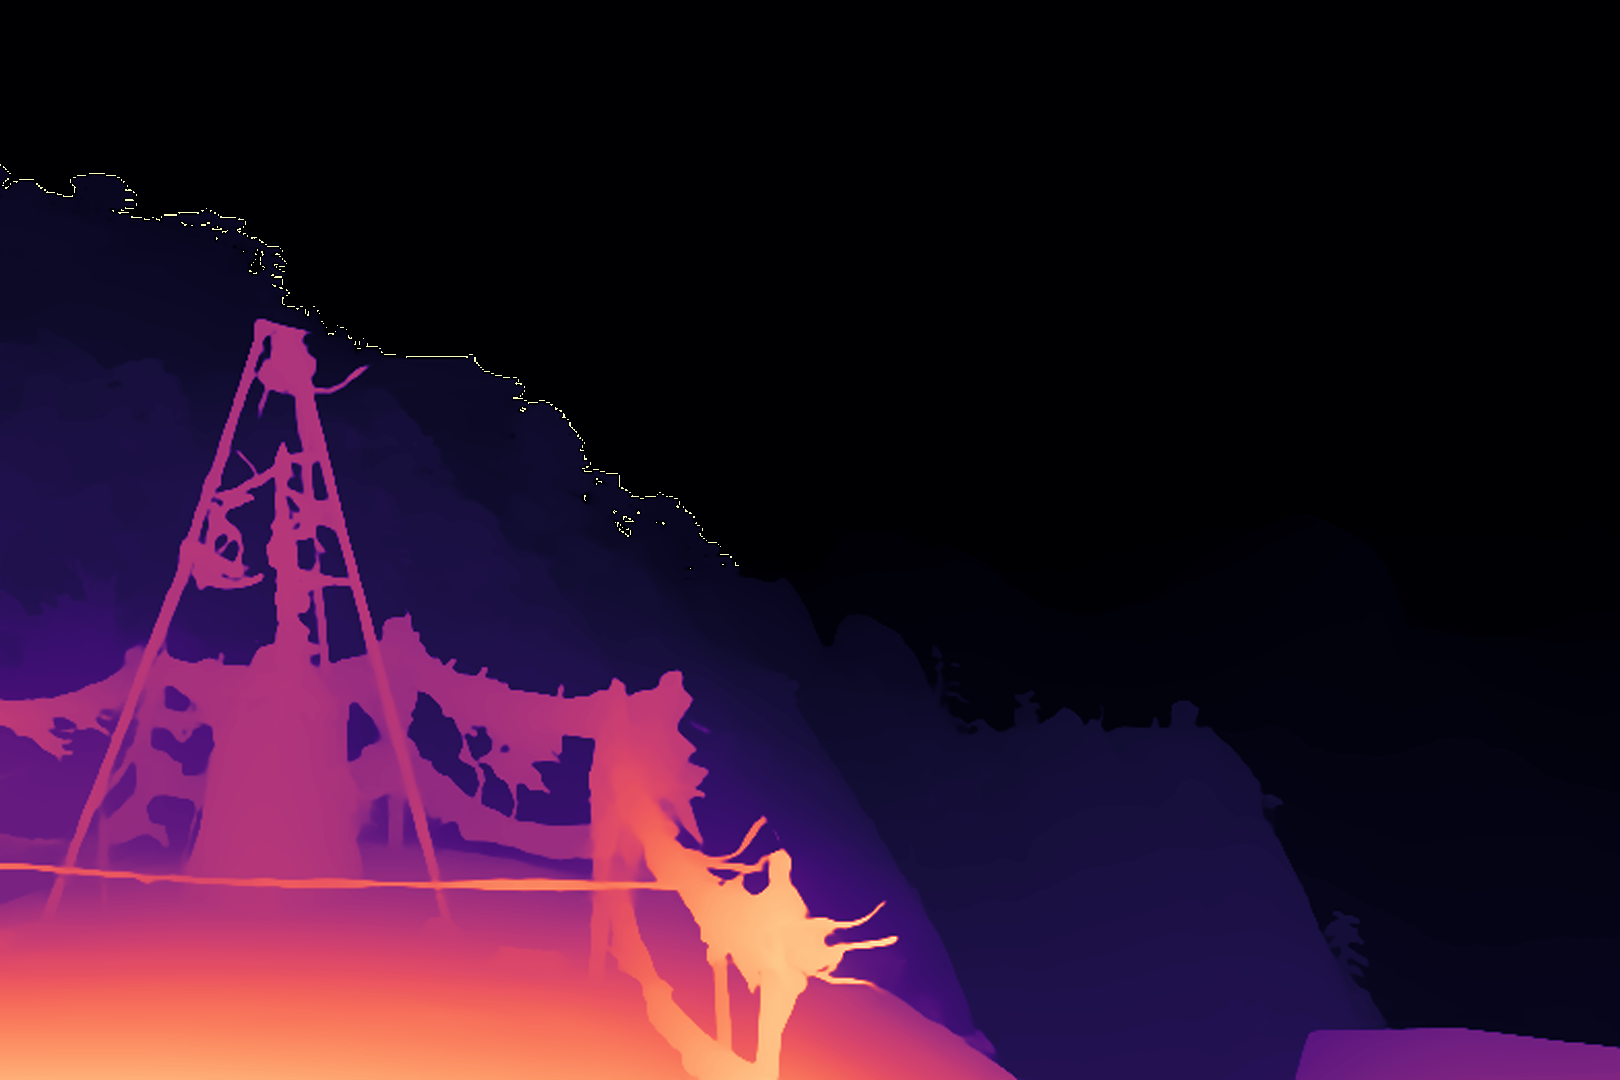
\includegraphics[width=0.49\textwidth]{./figures/huashan_depthmap.png}
        \caption{Sample Input $\to$ Output (V2, large model)}
        \label{fig:intro}
    \end{figure}

\end{frame}

%have a teacher, student model; with segmentation
\begin{frame}
    \frametitle{Architecture V1}
    \framesubtitle{Overview}
    
    \begin{columns}
        
        \column{0.4\textwidth}
        
        \textbf{Datasets}
        \begin{equation*}
            \begin{aligned}
                \underbrace{\mathcal{D}^l}_{\text{labeled}} &= 
                \begin{cases} 
                    \text{6 Datasets} \\ 
                    \text{1.5M Images} 
                \end{cases} \\
                \underbrace{\mathcal{D}^u}_{\text{unlabeled}} &= 
                \begin{cases} 
                    \text{8 Datasets} \\ 
                    \text{62M Images} 
                \end{cases}
            \end{aligned}
        \end{equation*}
        \pause
        \begin{itemize}
            \item[Key] MiDaS $\leadsto$ Loss Function
        \end{itemize}
        
        
        \column{0.6\textwidth}
        \pause
        \textbf{Training Process}
        \begin{enumerate}
            \item<4-> Training Teacher $T$ with $\mathcal{D}^l$
            
            \item<5-> Use $T$ to \underline{pseudo-label}:
            \\$\mathcal{D}^u \xlongrightarrow{T} \hat{\mathcal{D}}^u $
            
            \item<6-> Training Student $S$ with $\hat{\mathcal{D}}^u \cup \mathcal{D}^l$
        \end{enumerate}
    
    \end{columns}
\end{frame}



\begin{frame}
    \frametitle{Architecture V1}
    \framesubtitle{Details}
    
    \begin{columns}
        \column{0.4\textwidth}
        \begin{tikzpicture}[node distance=2cm]
            
            % Nodes
             \node (startImage) [imageblock] {\includegraphics[width=2cm]{./figures/tianjin_orig.JPG}};
            \node (perturbations) [process, below of=startImage, yshift=0.8cm] {\small Perturbations};
            \node (imageMiddle) [imageblock, below of=perturbations, yshift=+0.8cm] {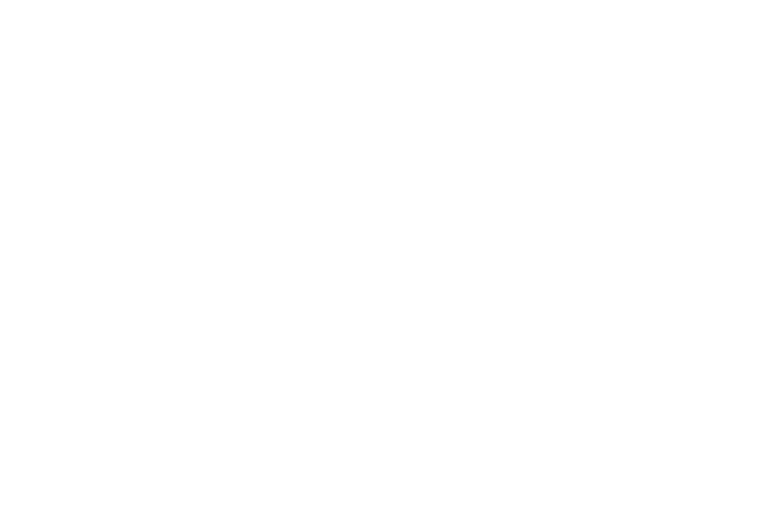
\includegraphics[width=2cm]{./figures/cutmix_example.png}};
            \node (encoderStatic) [process, below of=imageMiddle, yshift=0.8cm, xshift=-1.3cm] {\small Encoder Static};
            \node (encoderDynamic) [process, below of=imageMiddle, yshift=0.8cm, xshift=1.3cm] {\small Encoder};
            \node (decoder) [process, below of=encoderStatic, yshift=1.2cm, xshift=1.3cm] {\small Decoder};
            \node (imageEnd) [imageblock, below of=decoder, yshift=+0.8cm] {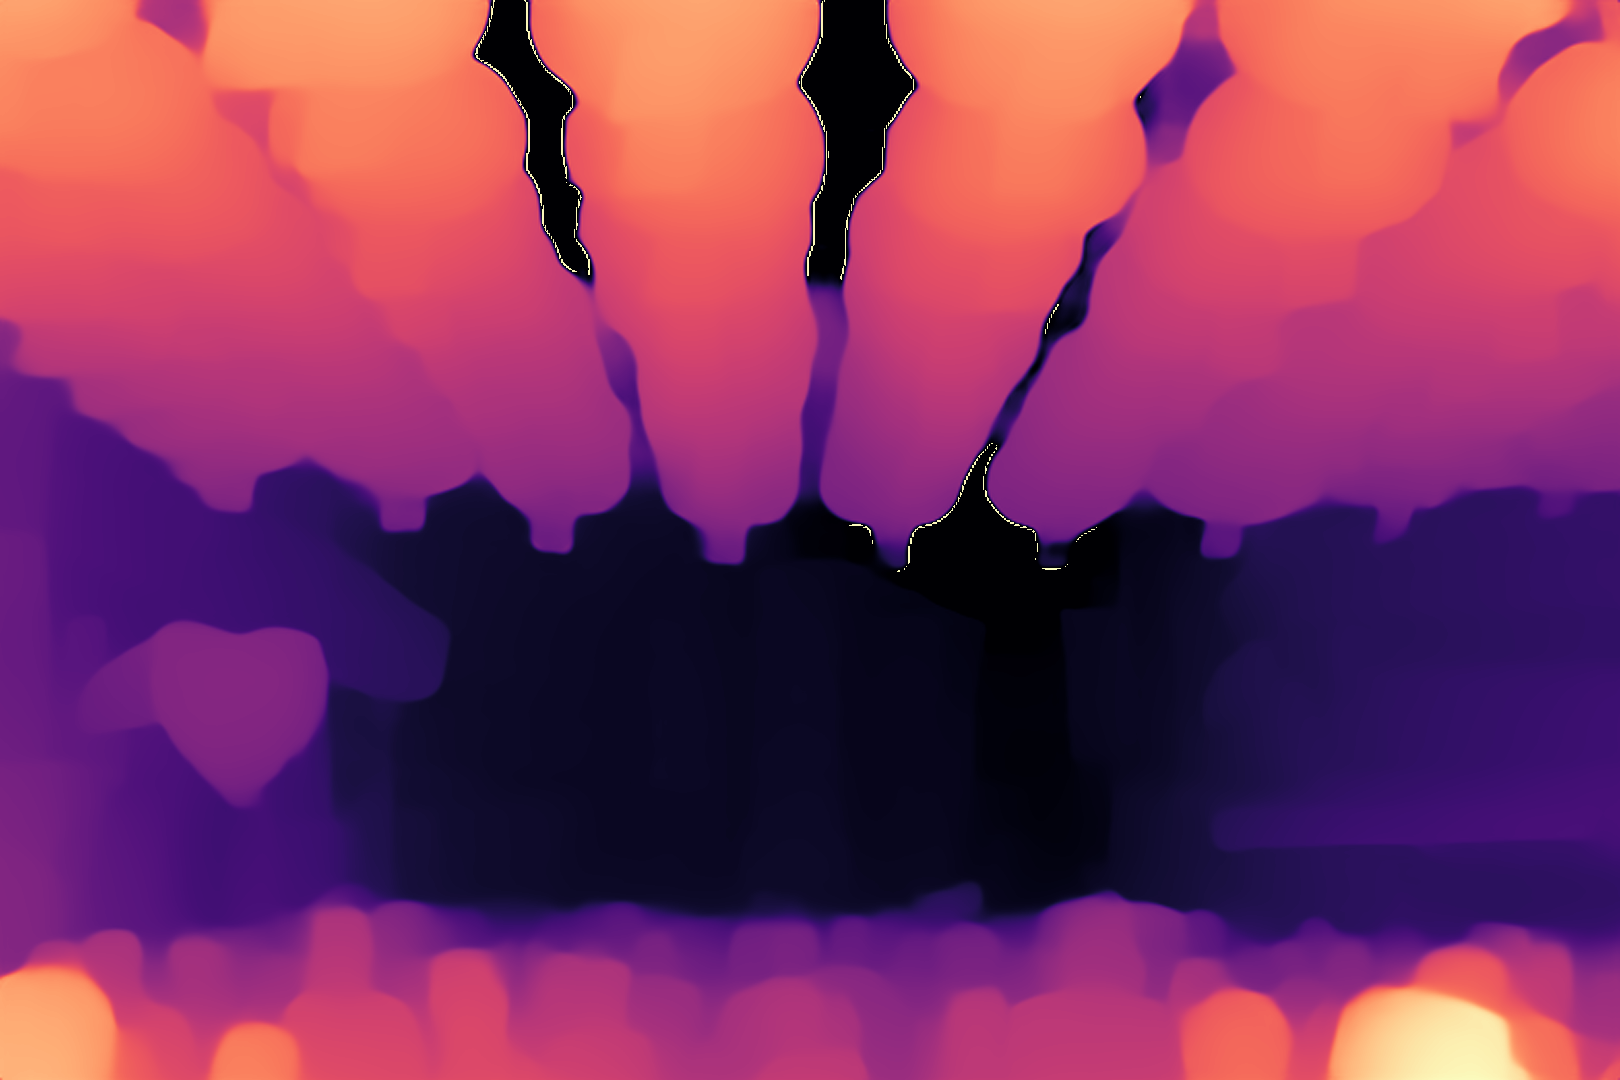
\includegraphics[width=2cm]{./figures/tianjin_depthmap_v1-small.png}};
            
            % Arrows
            \draw [arrow] (startImage) -- (perturbations);
            \draw [arrow] (perturbations) -- (imageMiddle);
            \draw [arrow] (imageMiddle) -- (encoderStatic);
            \draw [arrow] (imageMiddle) -- (encoderDynamic);
            \draw [arrow] (encoderDynamic) -- (decoder);
            \draw [arrow] (encoderStatic) -- (decoder);
            \draw [arrow] (decoder) -- (imageEnd);
            
        \end{tikzpicture}
    
        \column{0.6\textwidth}
        \pause
        
        \begin{itemize}
            \item<2-> Perturbations (only for $S$)
            \begin{itemize}
                \item[$\in\hat{\mathcal{D}}^u$] color shift + CutMix
                \item[$\in\mathcal{D}^l$] horizontal flip
            \end{itemize}
            $\leadsto$ be more robust
        
            \item<3-> Encoders
            \begin{itemize}
                \item[Normal] $\leftarrow$ DINOv2 encoder
                \item[Static] $\leftarrow$ frozen DINOv2 encoder
                \item Linked by a feature alignment loss
            \end{itemize}
            $\leadsto$ auxiliary supervision
            
            \item<4-> Decoder $\leftarrow$ DPT decoder (as in MiDaS)
            
        \end{itemize}
    \end{columns}
    
\end{frame}

\begin{frame}
    \frametitle{Architecture V2}
    
    \textbf{Situation}
    \begin{itemize}
        \item[Problem] real labels are \underline{inaccurate} $\leadsto$ no fine detail in V1
        \item[Idea] Use \underline{synthetic images} to train $T$
    \end{itemize}
    \pause
    \begin{figure}
        \centering
        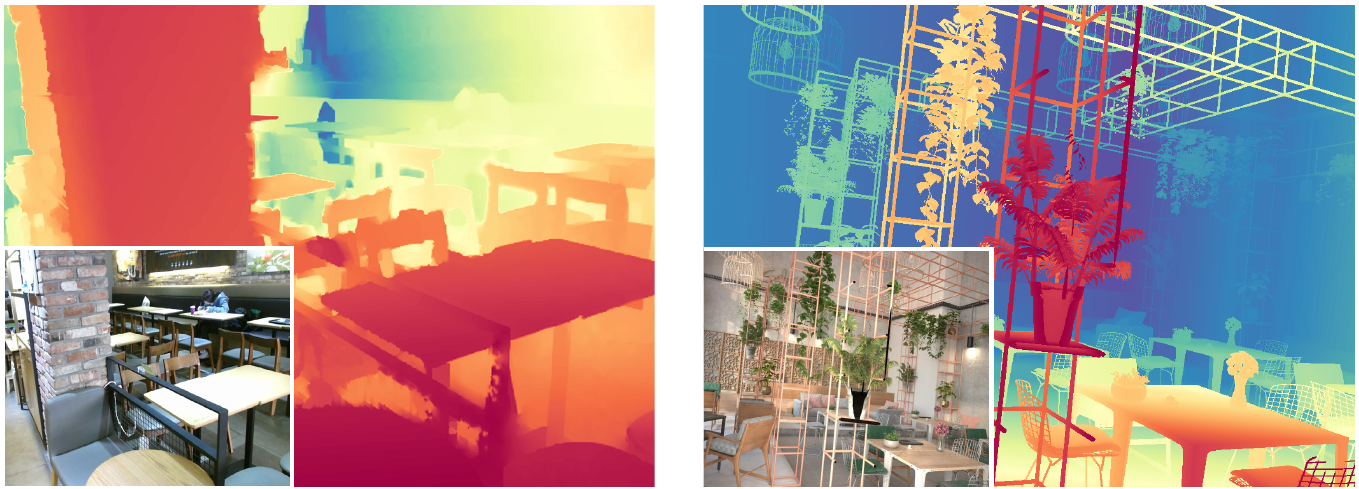
\includegraphics[width=\textwidth]{./figures/screeenshot_deepanythingv2_realvssynth.png}
        \caption{From Deep Anything V2: Example of real label (left), synthetic label (right)}
        \label{fig:realvssynth}
    \end{figure}
\end{frame}

\begin{frame}
    \textbf{Synthetic Images}
    \begin{columns}
        \column{0.5\textwidth}
        \begin{itemize}
            \item[+] Fine Details
            \item[+] Transparent, Reflective Surfaces
        \end{itemize}
        \column{0.5\textwidth}
        \begin{itemize}
            \item[-] Not photorealistic
            \item[-] Limited Scenes
        \end{itemize}
    \end{columns}

    \vspace{0.5cm}
    \pause
    
    \textbf{Solution: Modify Training Process}
    \begin{enumerate}
        \item<2-> Training Teacher $T$ with \cancel{$\mathcal{D}^l$}  $\mathcal{D}^l_s$
        \begin{itemize}
            \item $\mathcal{D}^l_s$ ... labeled synthetic dataset
            \item fewer images ($\approx$ 0.6M)
            \item based on DINOv2 Giant
        \end{itemize}

        
        \item<3-> Use $T$ to \underline{pseudo-label}:
        \\$\mathcal{D}^u \xlongrightarrow{T} \hat{\mathcal{D}}^u $
        
        \item<4-> Training Student $S$ with \cancel{$\hat{\mathcal{D}}^u \cup \mathcal{D}^l$} $\hat{\mathcal{D}}^u$
    \end{enumerate}
    
\end{frame}


%quantative and qualitative results; note that fine details hard to compare
\begin{frame}
    \frametitle{Qualitative Results}
    
    \begin{figure}
        \centering
        \includegraphics[width=0.32\textwidth]{./figures/tianjin_orig.JPG}
        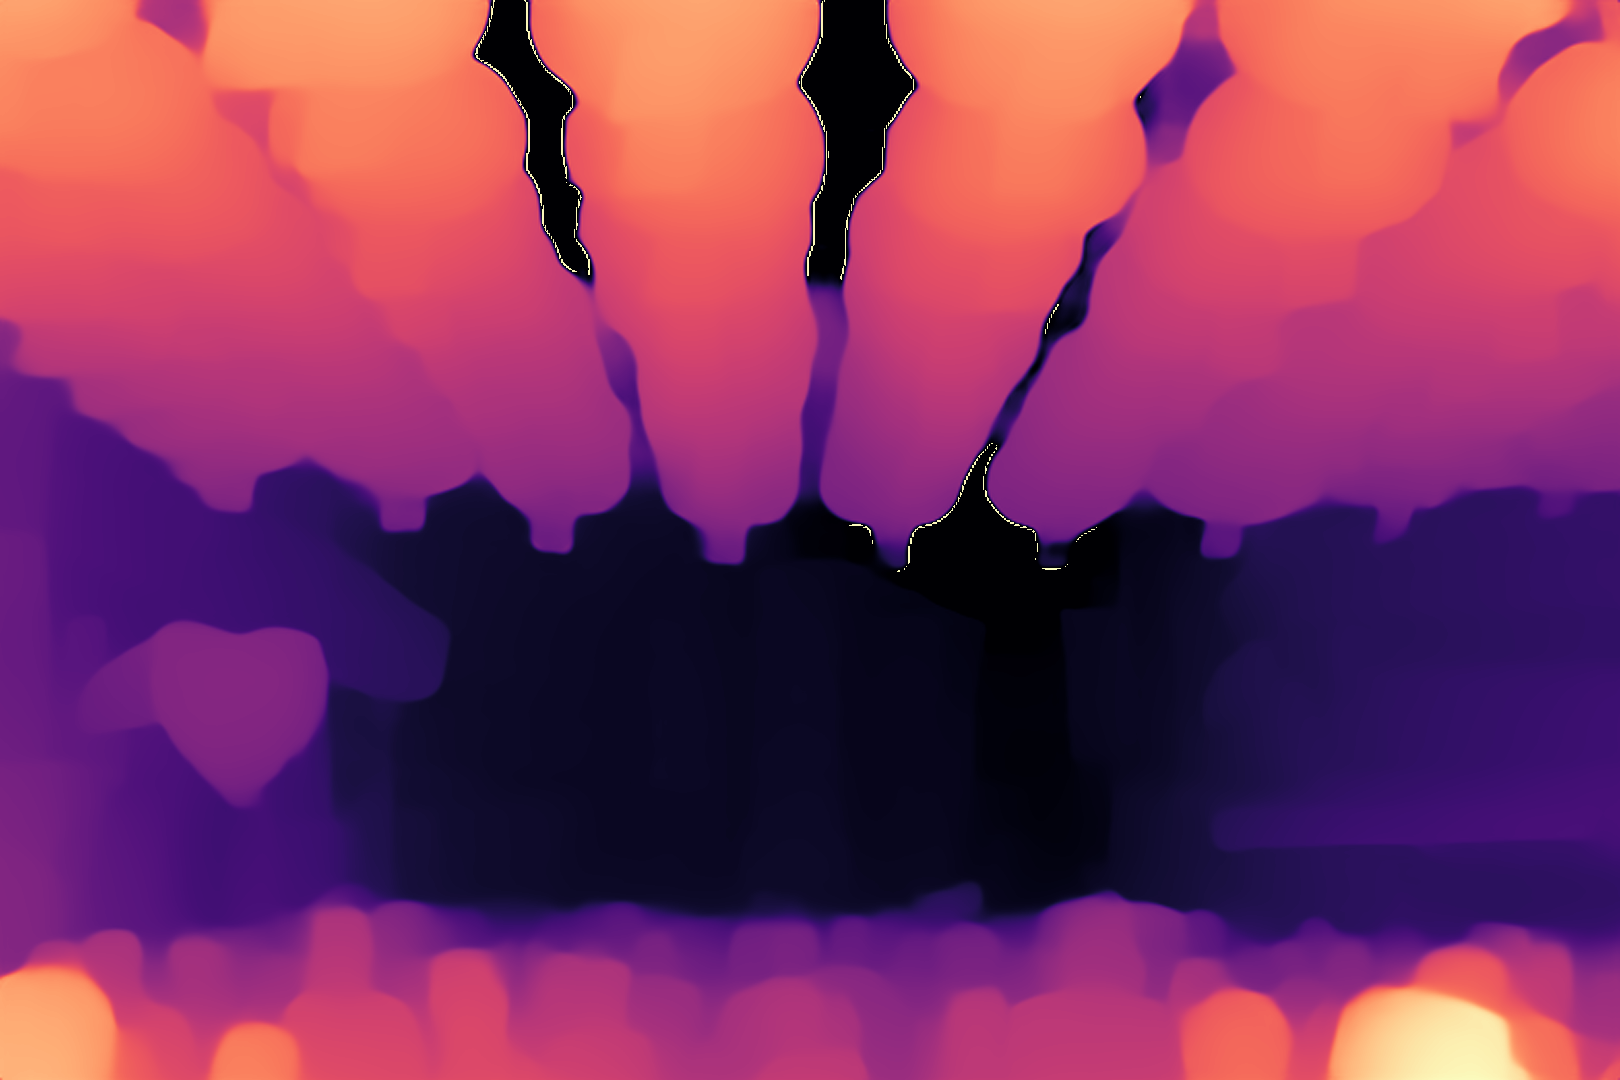
\includegraphics[width=0.32\textwidth]{./figures/tianjin_depthmap_v1-small.png}
        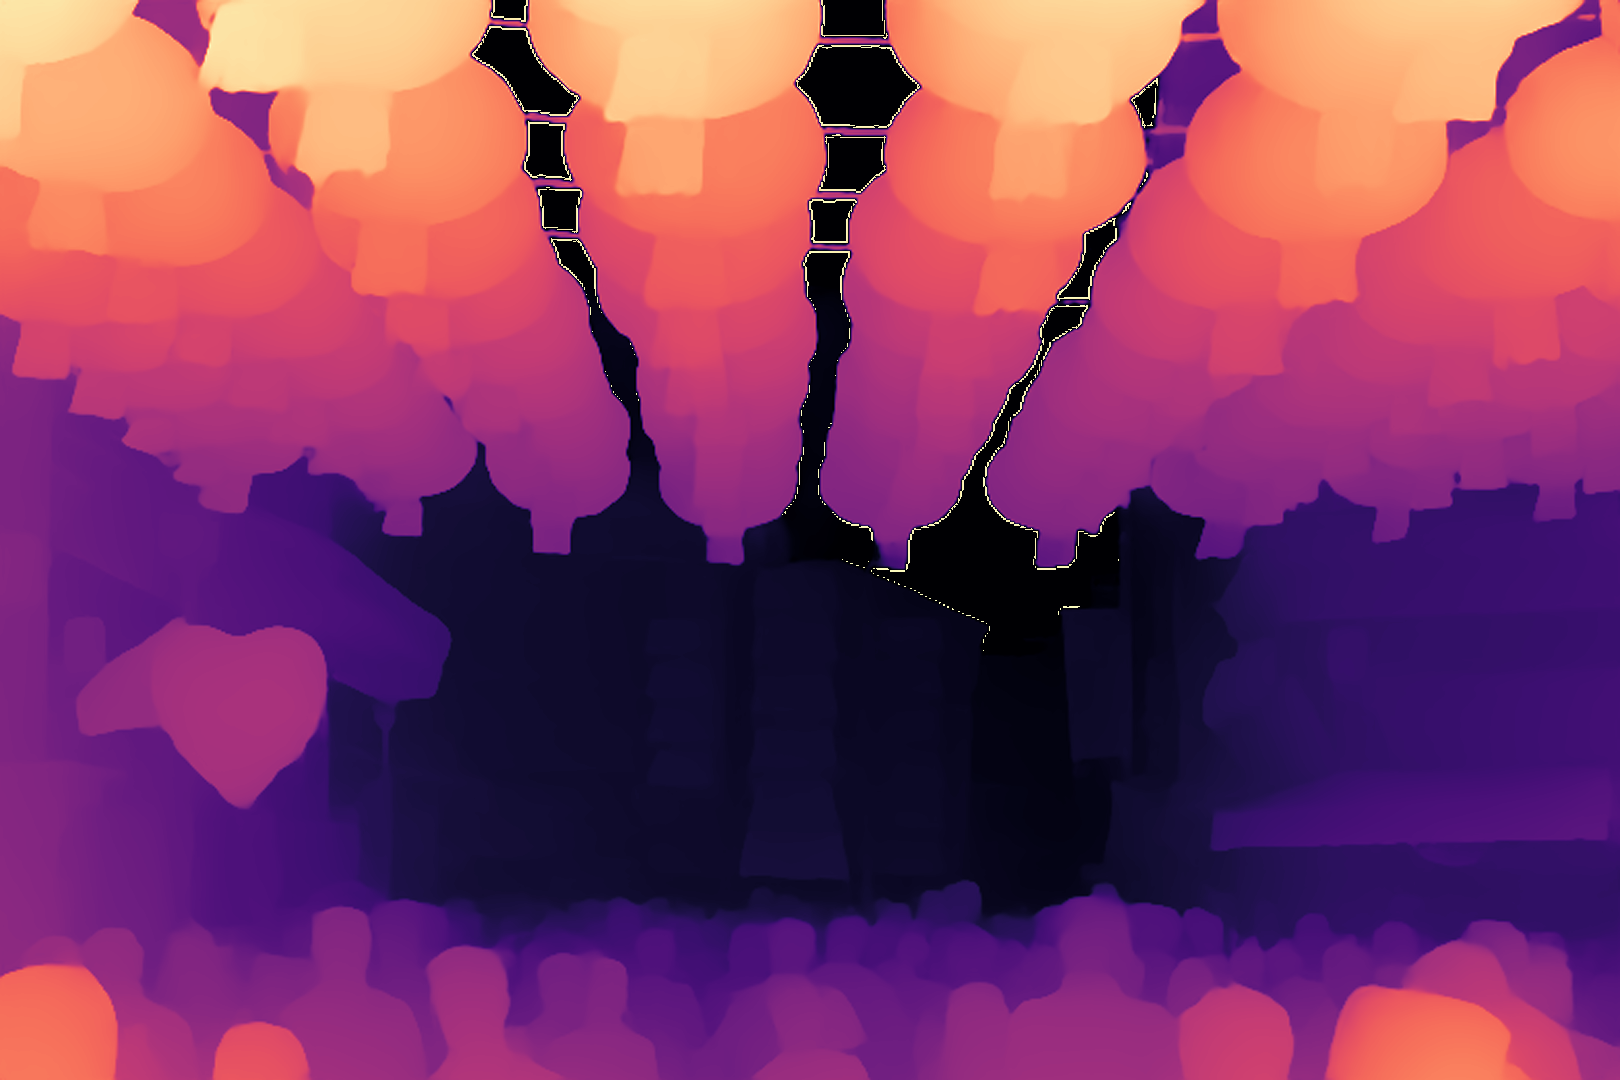
\includegraphics[width=0.32\textwidth]{./figures/tianjin_depthmap_v2-small.png}
        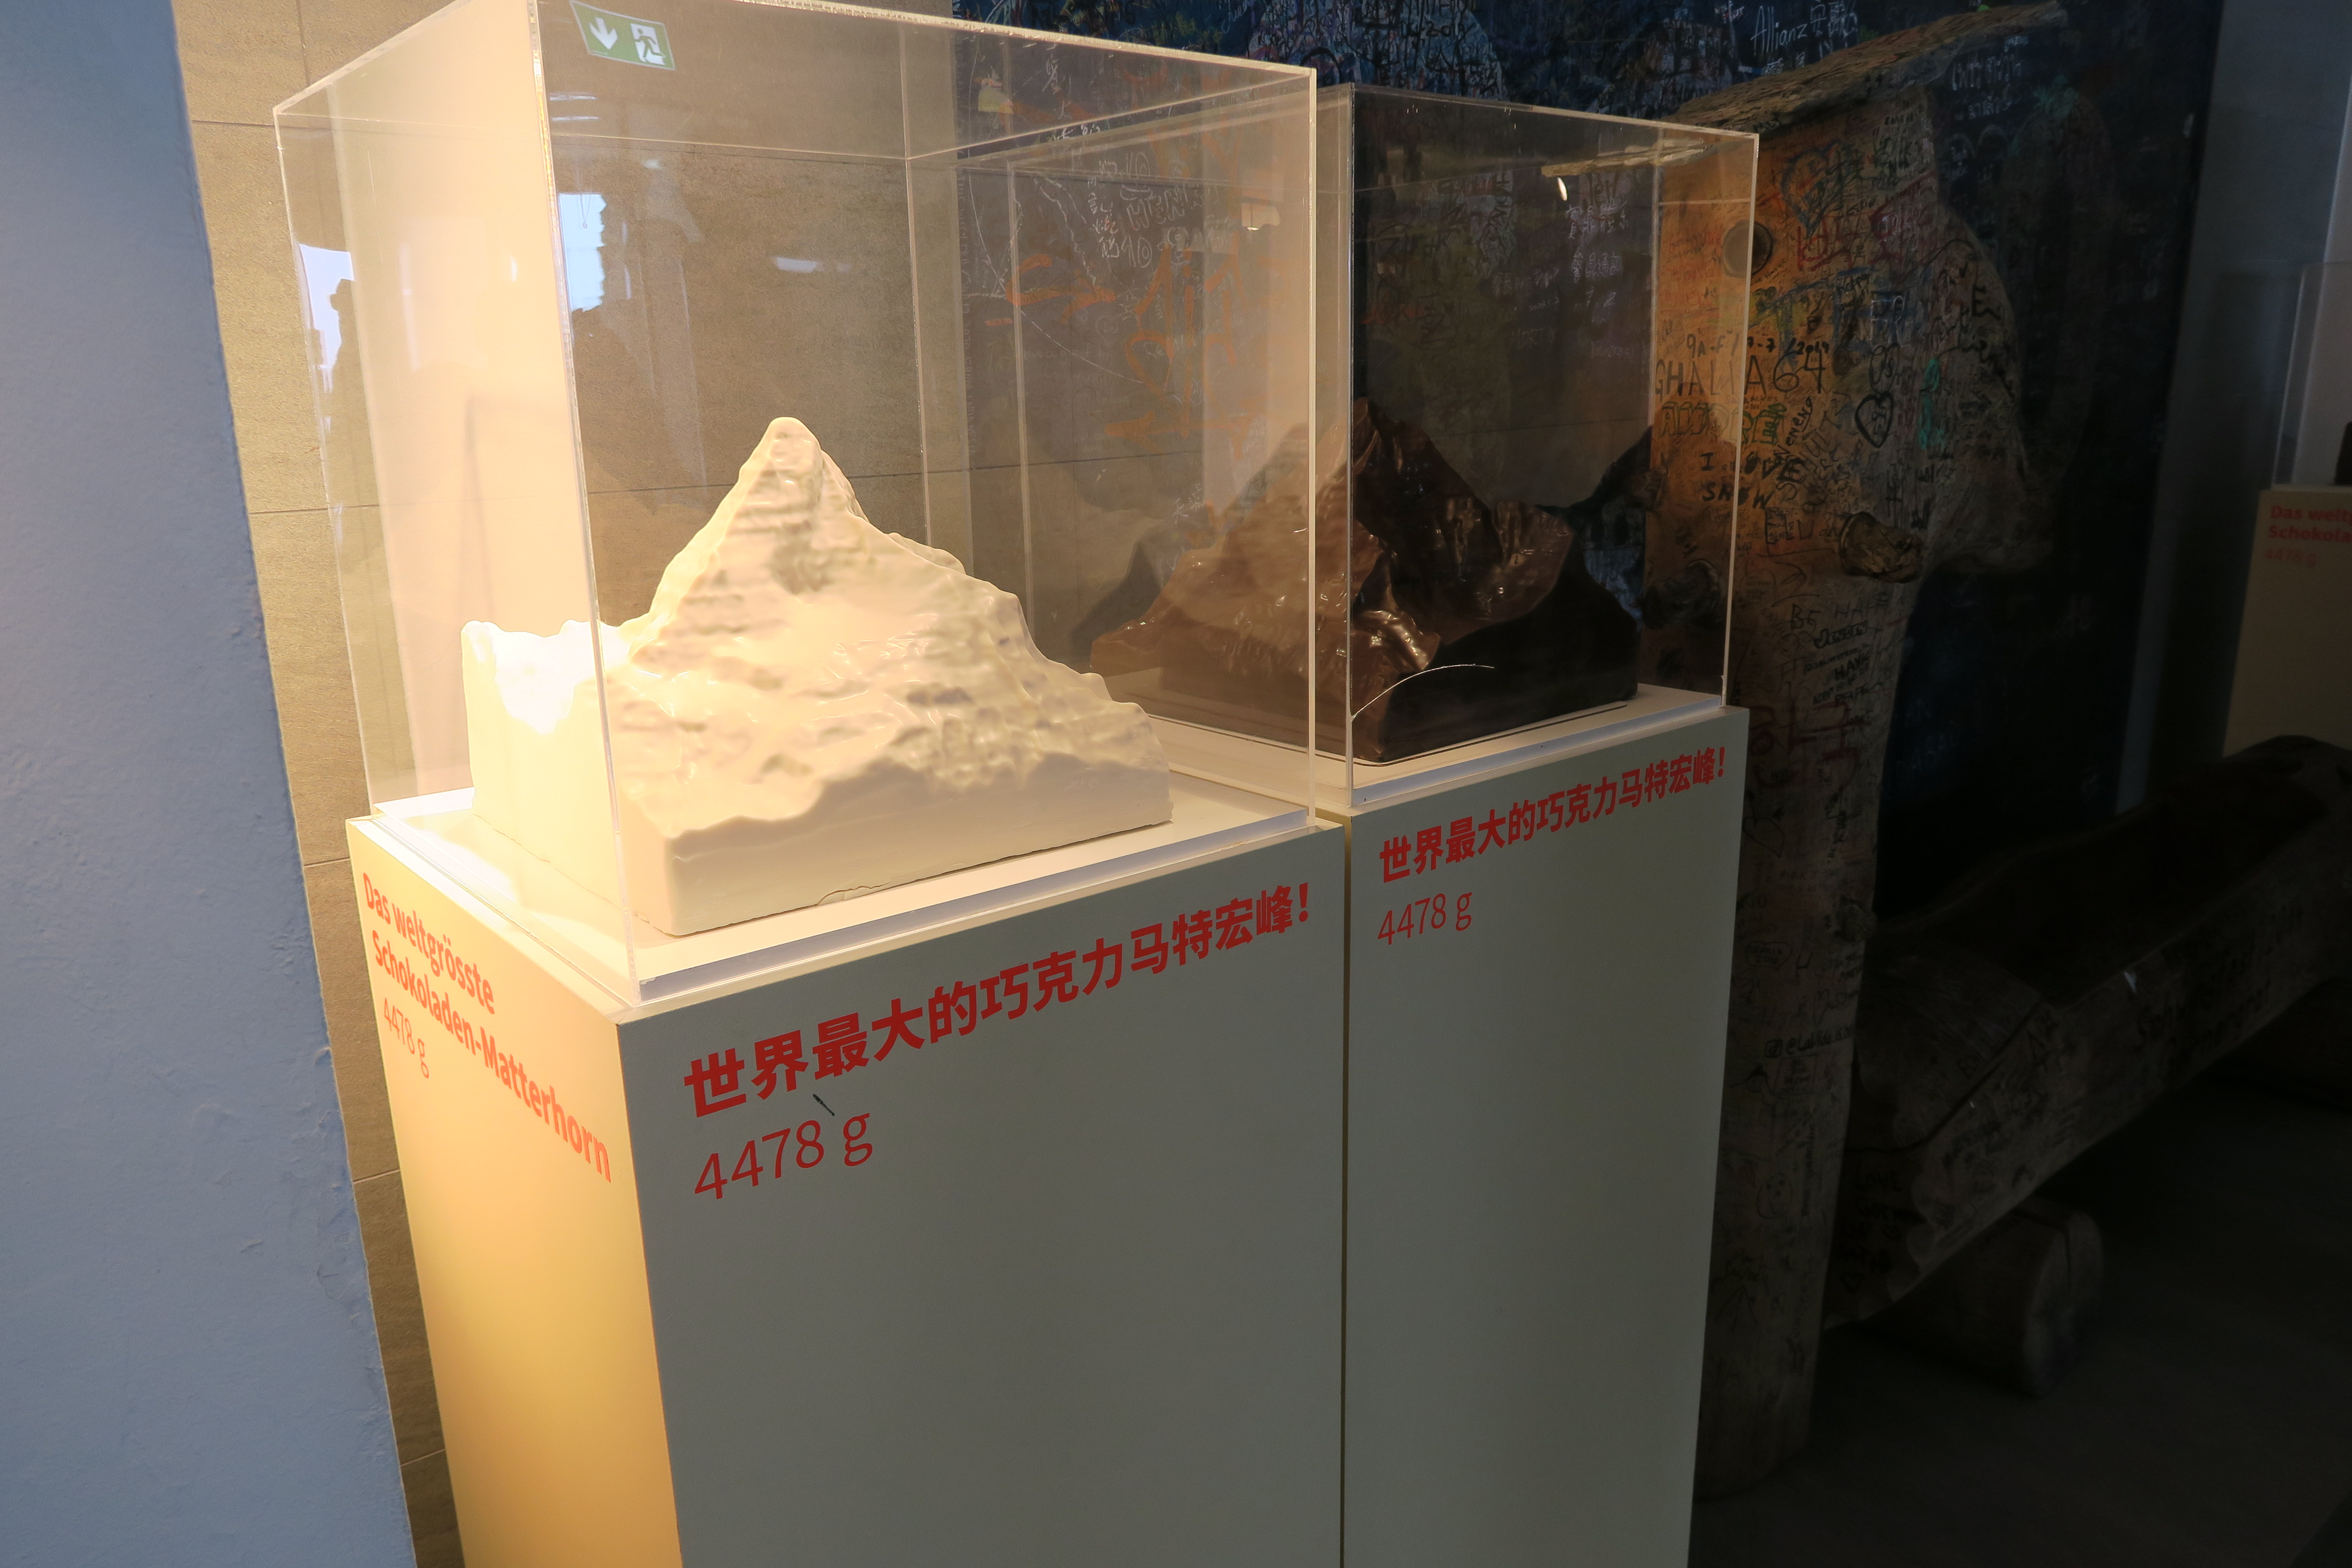
\includegraphics[width=0.32\textwidth]{./figures/schoggimatterhorn.JPG}
        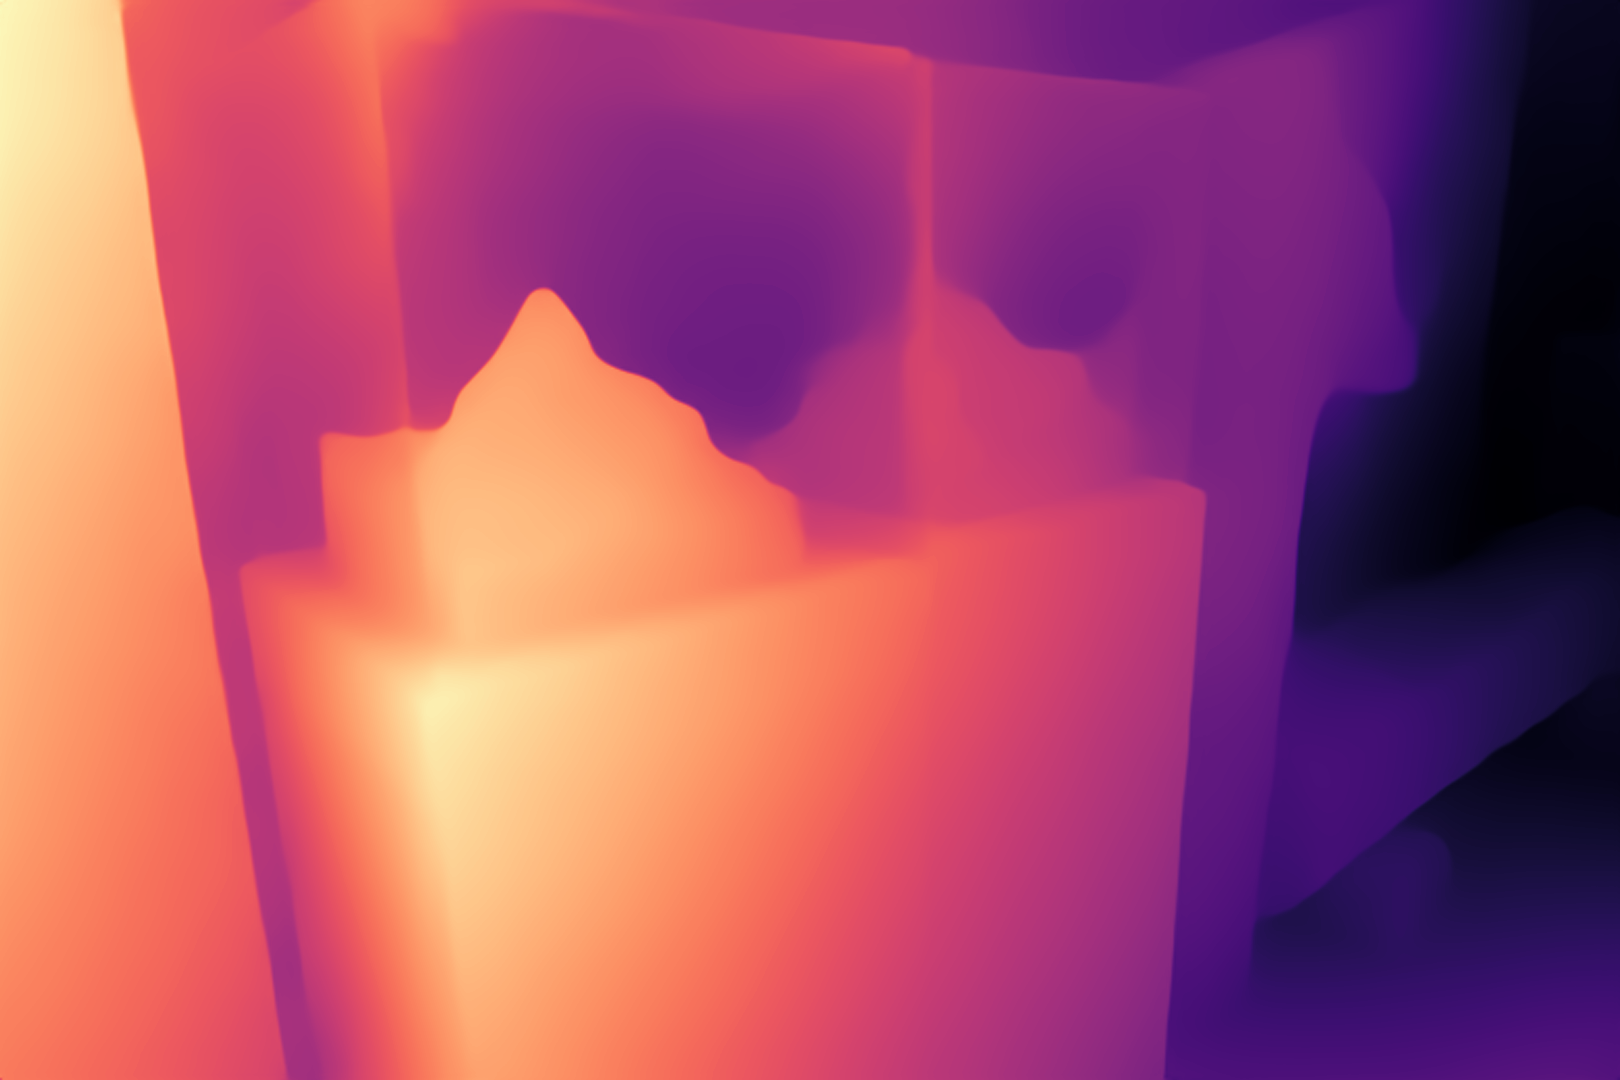
\includegraphics[width=0.32\textwidth]{./figures/schoggimatterhorn_v1-small.png}
        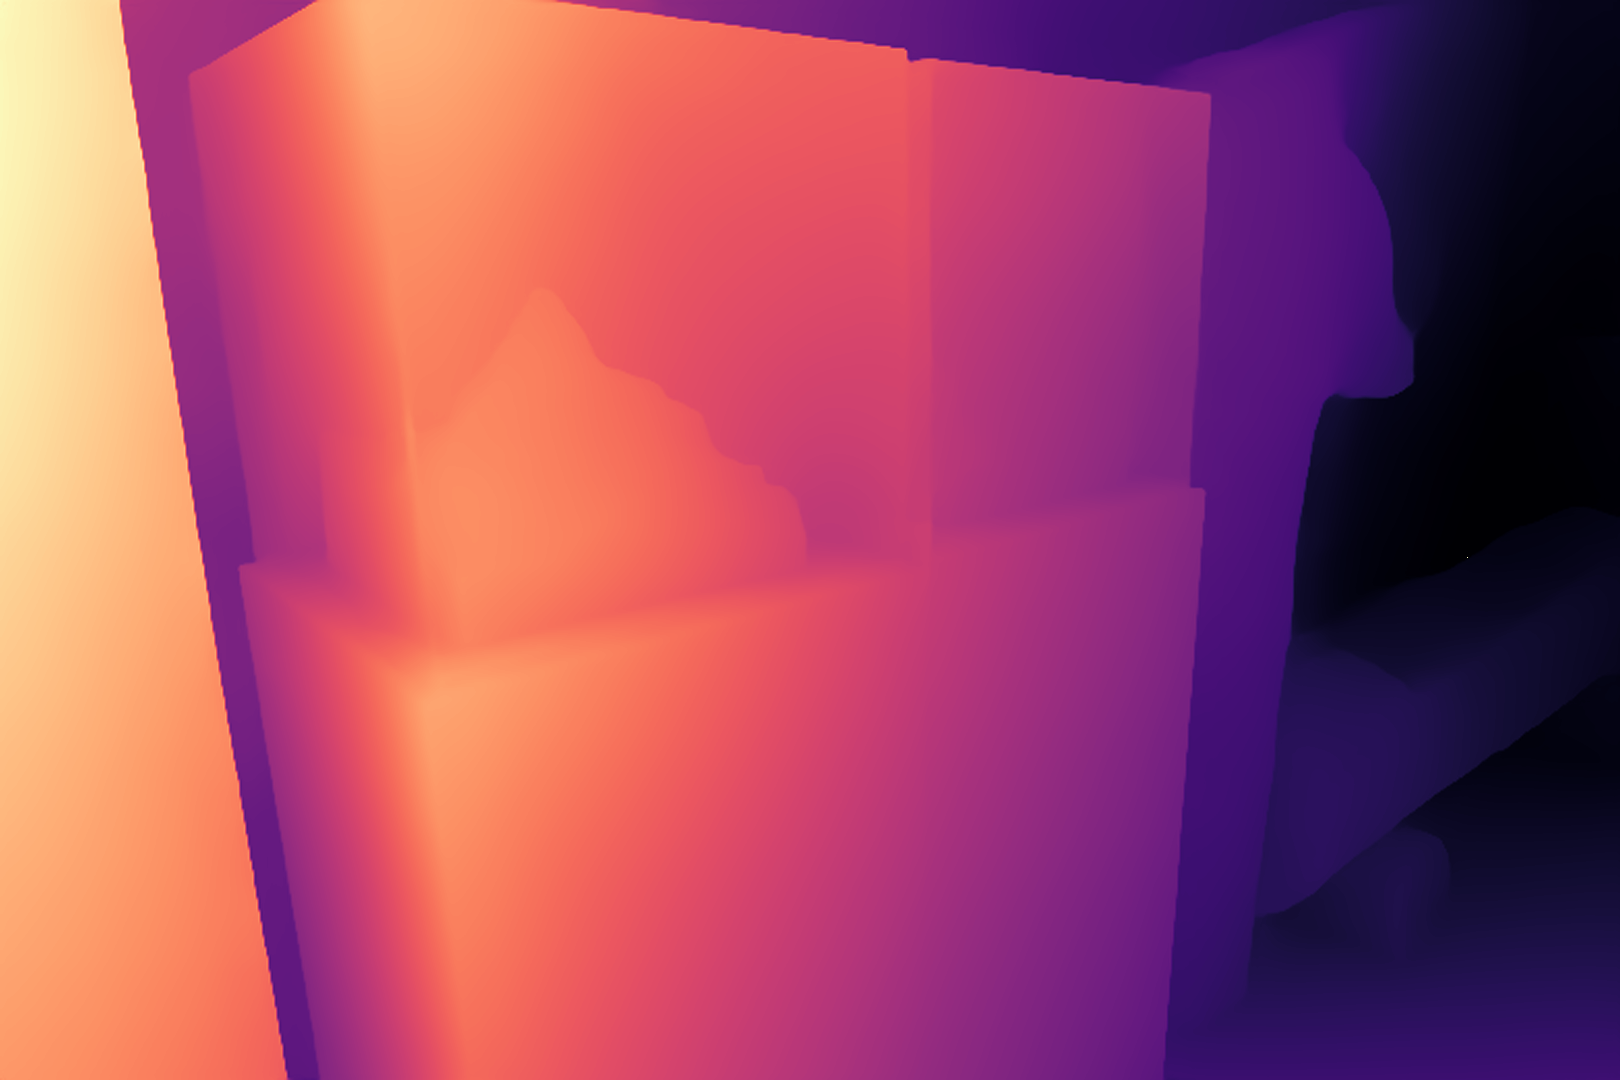
\includegraphics[width=0.32\textwidth]{./figures/schoggimatterhorn_v2-small.png}
        \includegraphics[width=0.32\textwidth]{./figures/gl_seeli.JPG}
        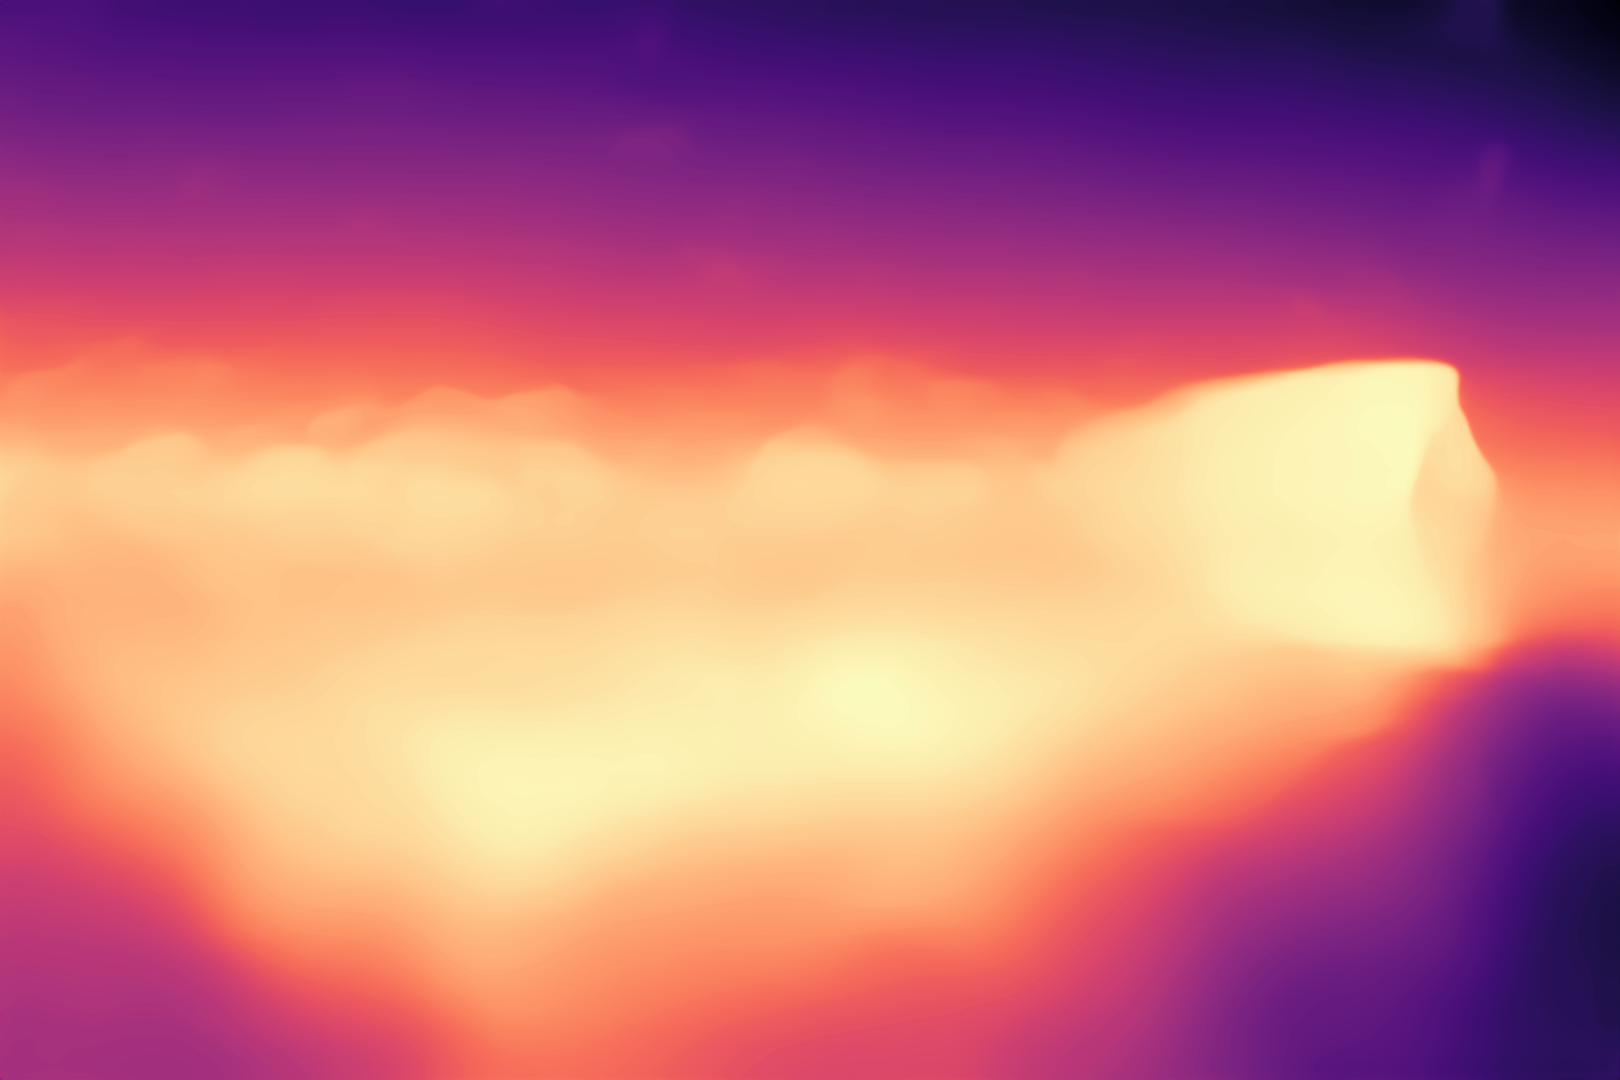
\includegraphics[width=0.32\textwidth]{./figures/gl_seeli_v1-small.png}
        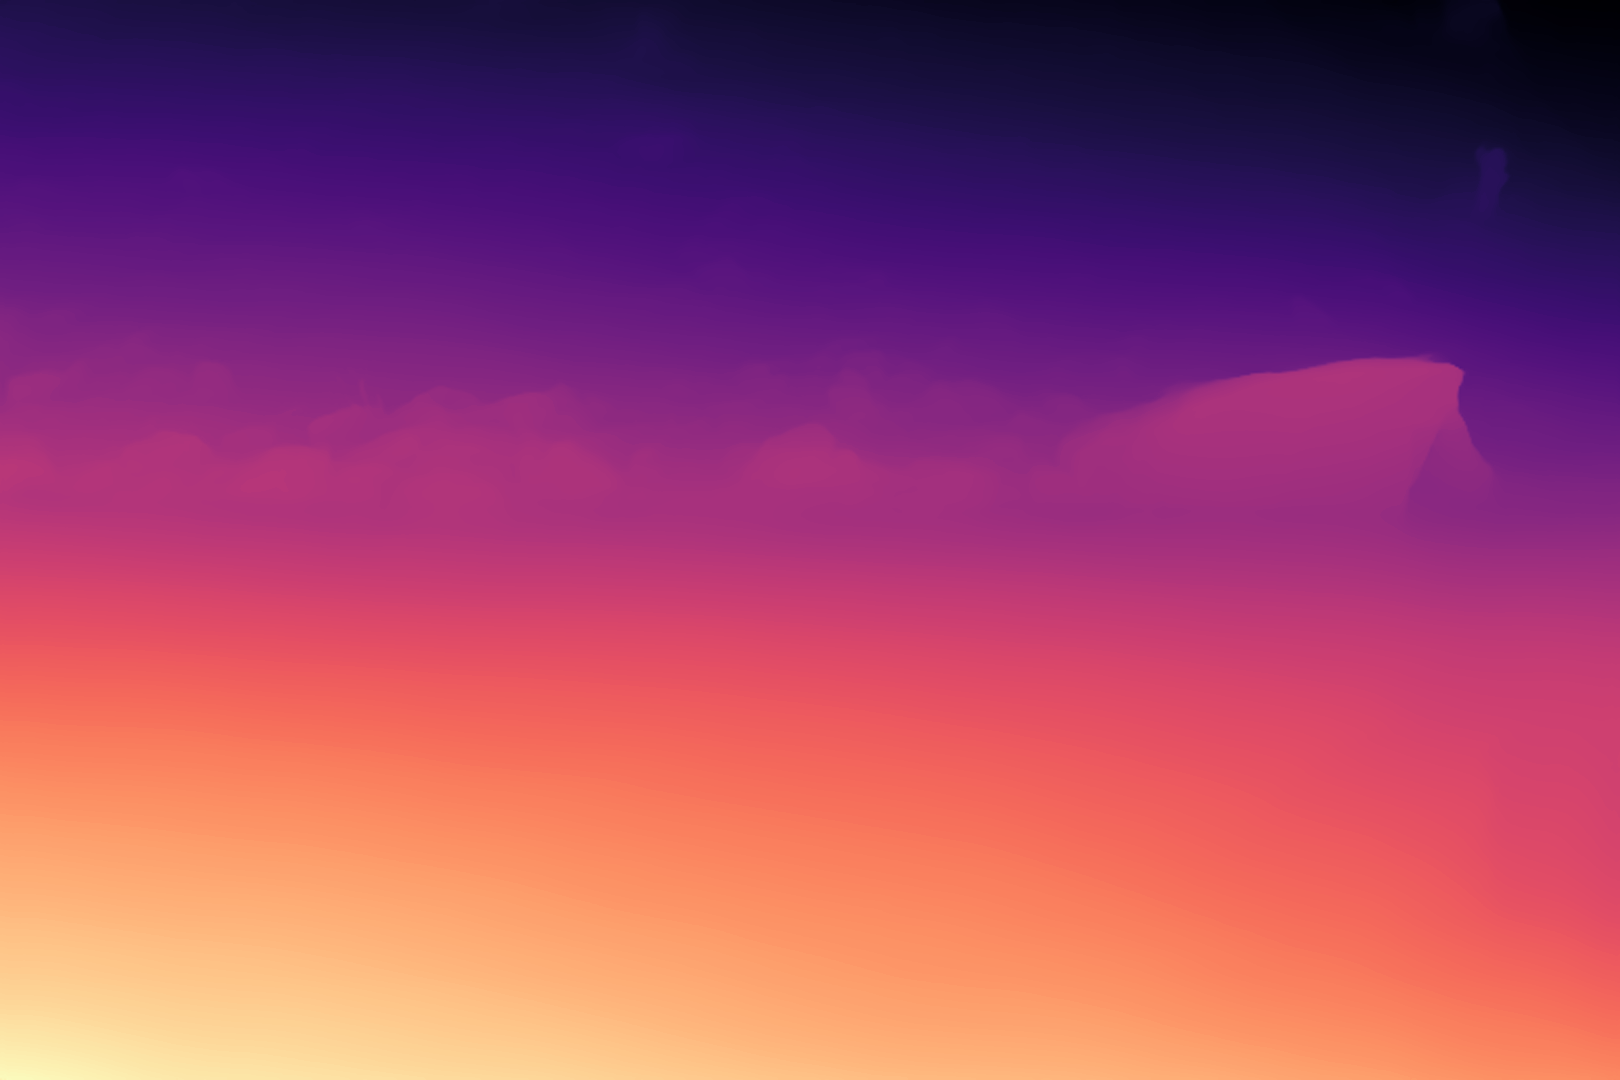
\includegraphics[width=0.32\textwidth]{./figures/gl_seeli_v2-small.png}
        \caption{Original (left), V1 (middle), and V2 (right) depth map}
        \label{fig:res_1}
    \end{figure}
\end{frame}

\begin{frame}
    \frametitle{Qualitative Results}
    
    \begin{figure}
        \centering
        \includegraphics[width=0.32\textwidth]{./figures/sbb_uw.JPG}
        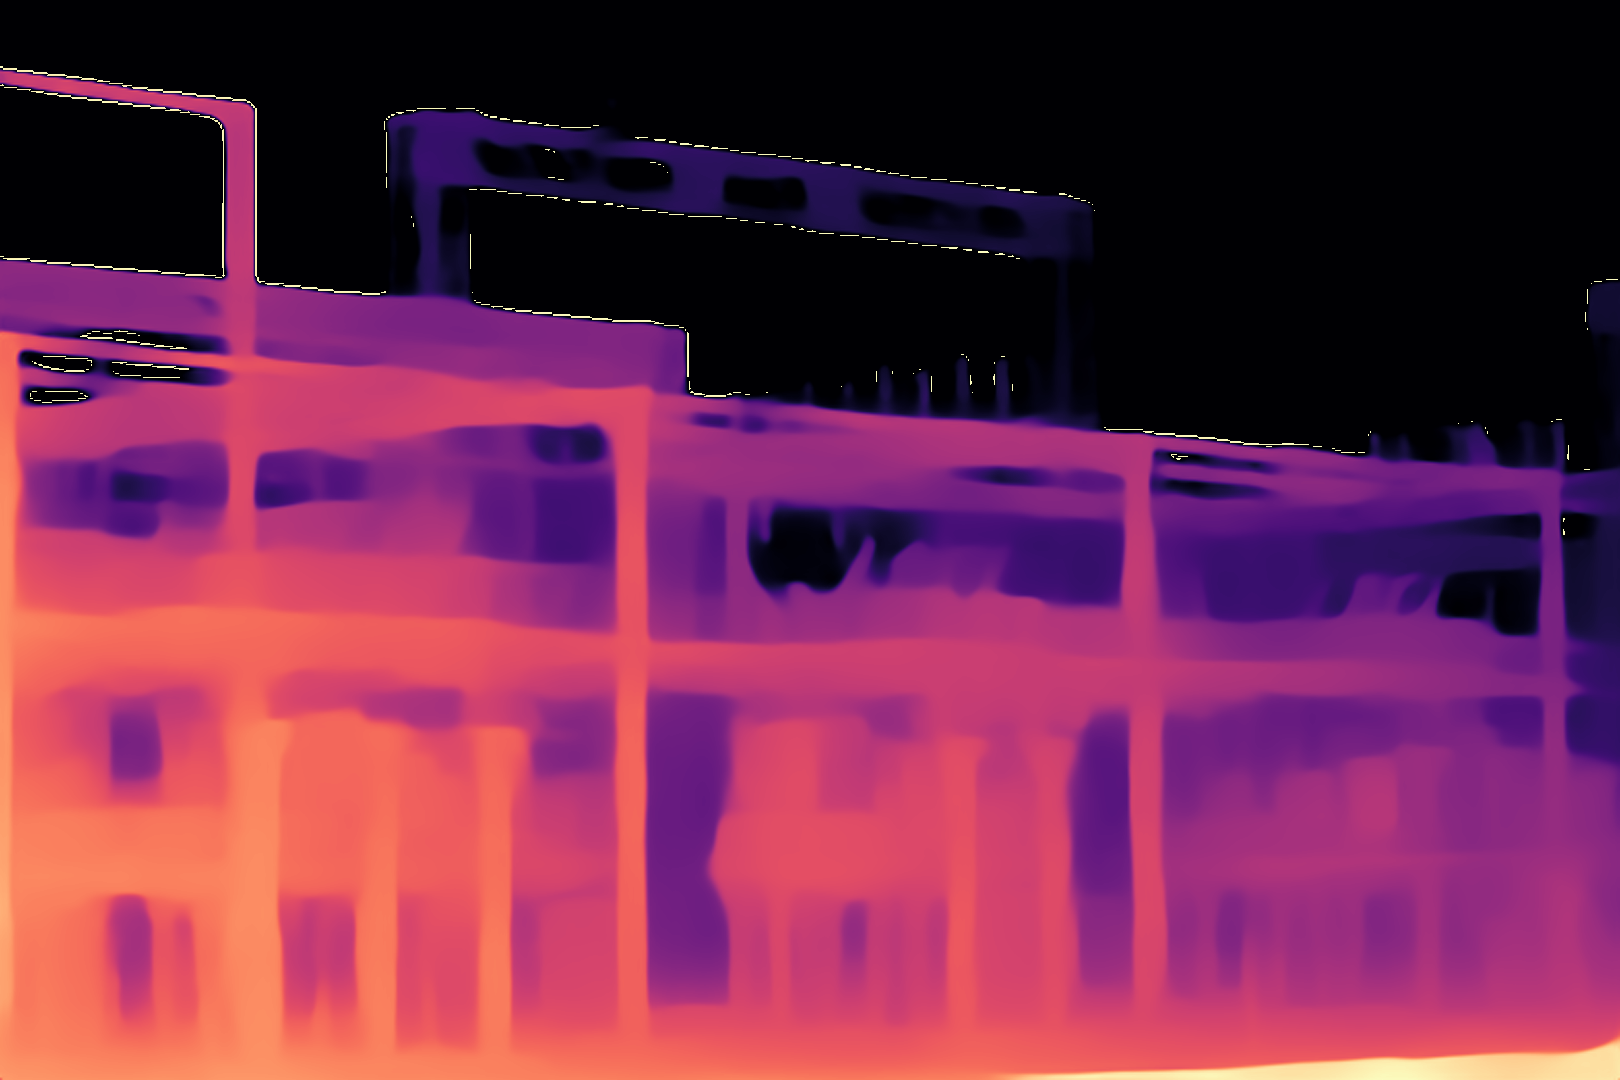
\includegraphics[width=0.32\textwidth]{./figures/sbb_uw_v1-small.png}
        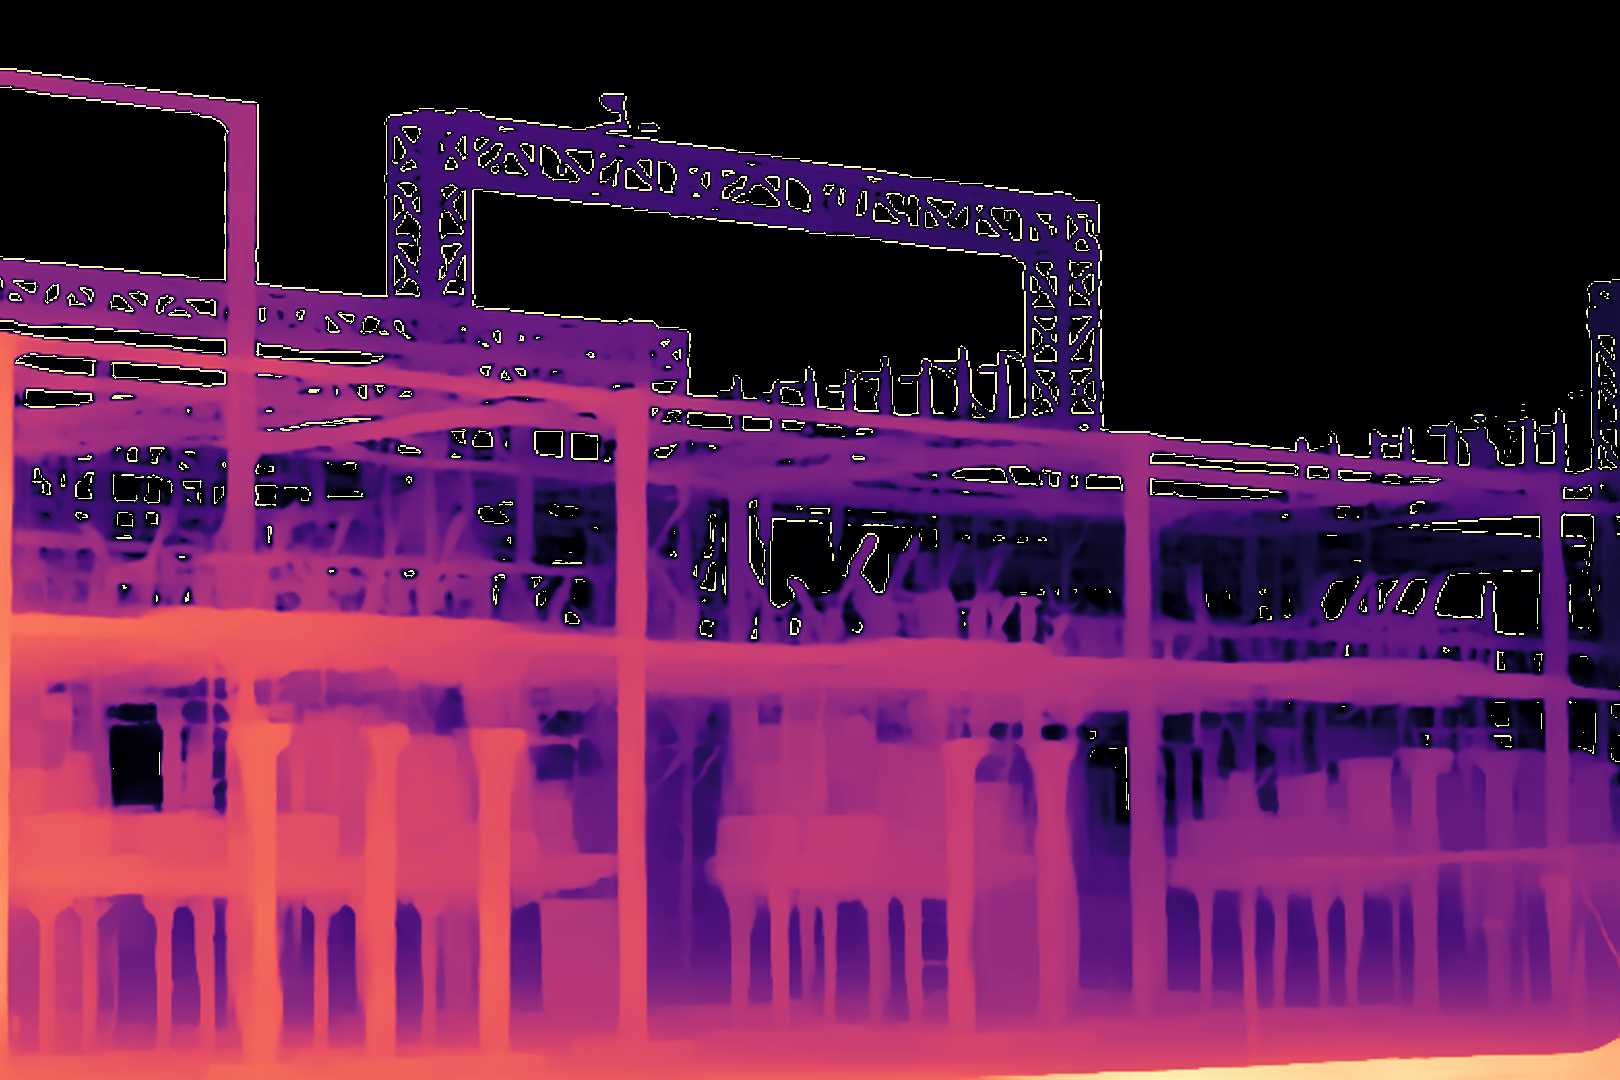
\includegraphics[width=0.32\textwidth]{./figures/sbb_uw_v2-small.png}
        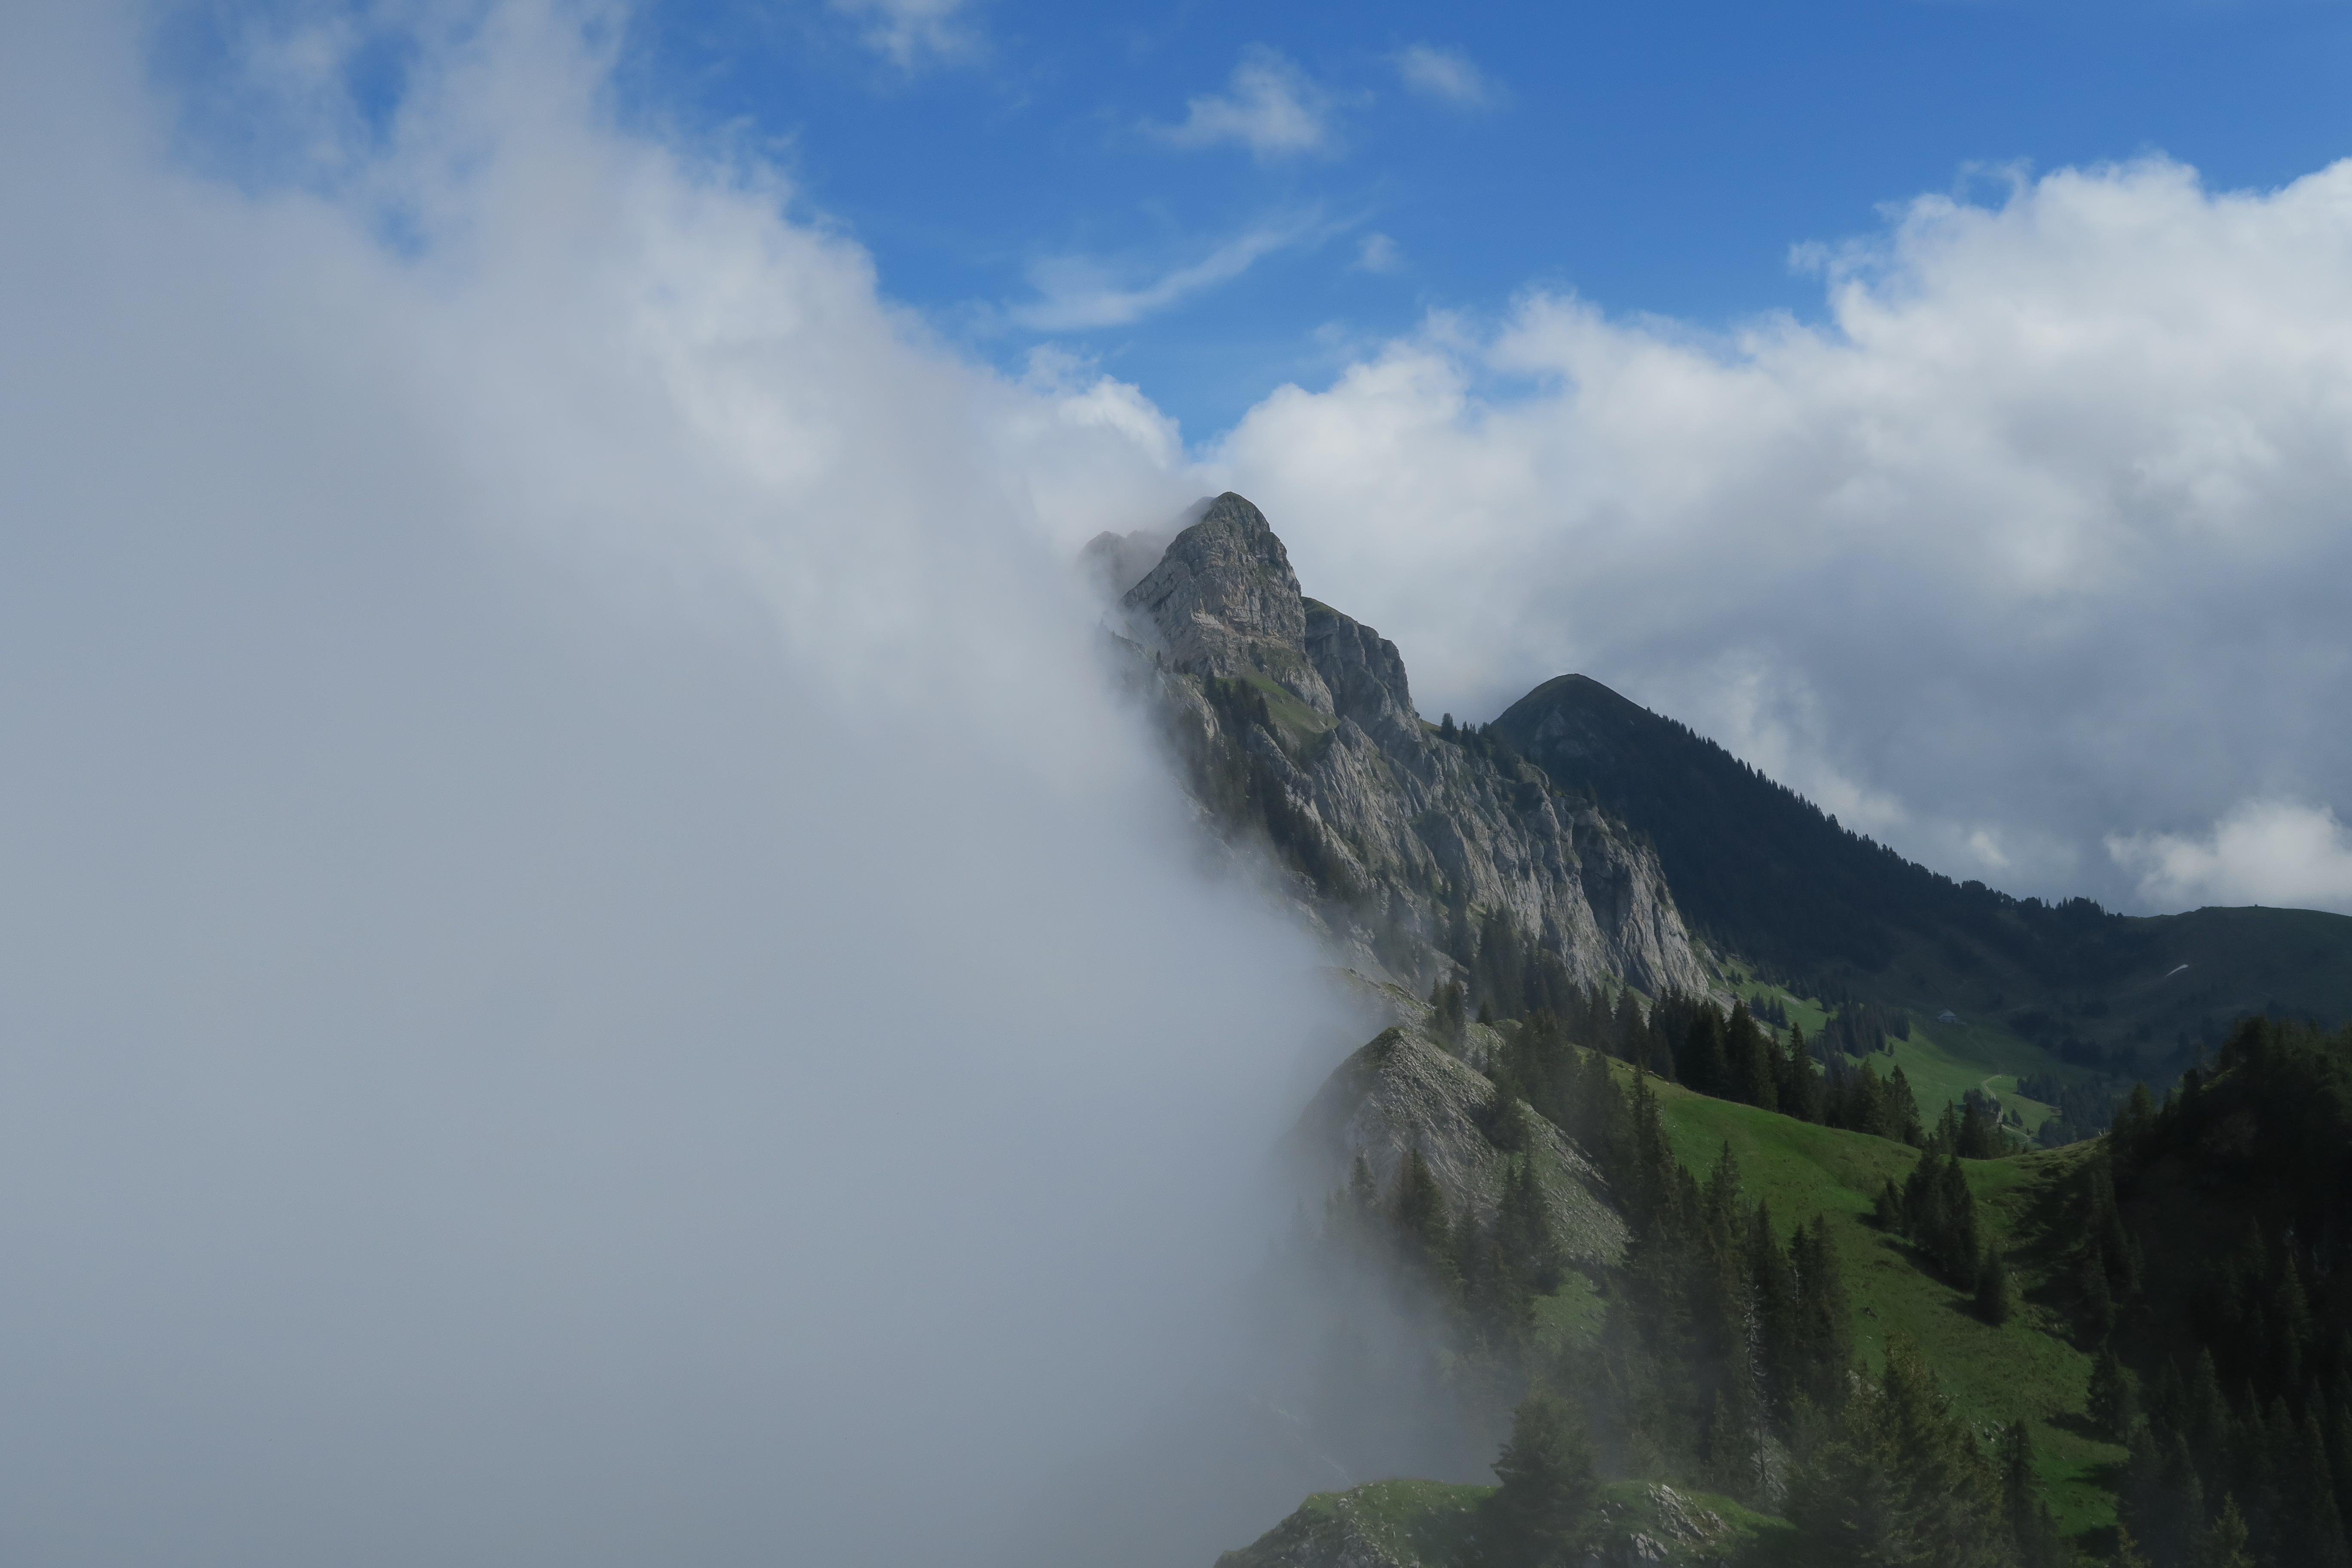
\includegraphics[width=0.32\textwidth]{./figures/luhinterland.JPG}
        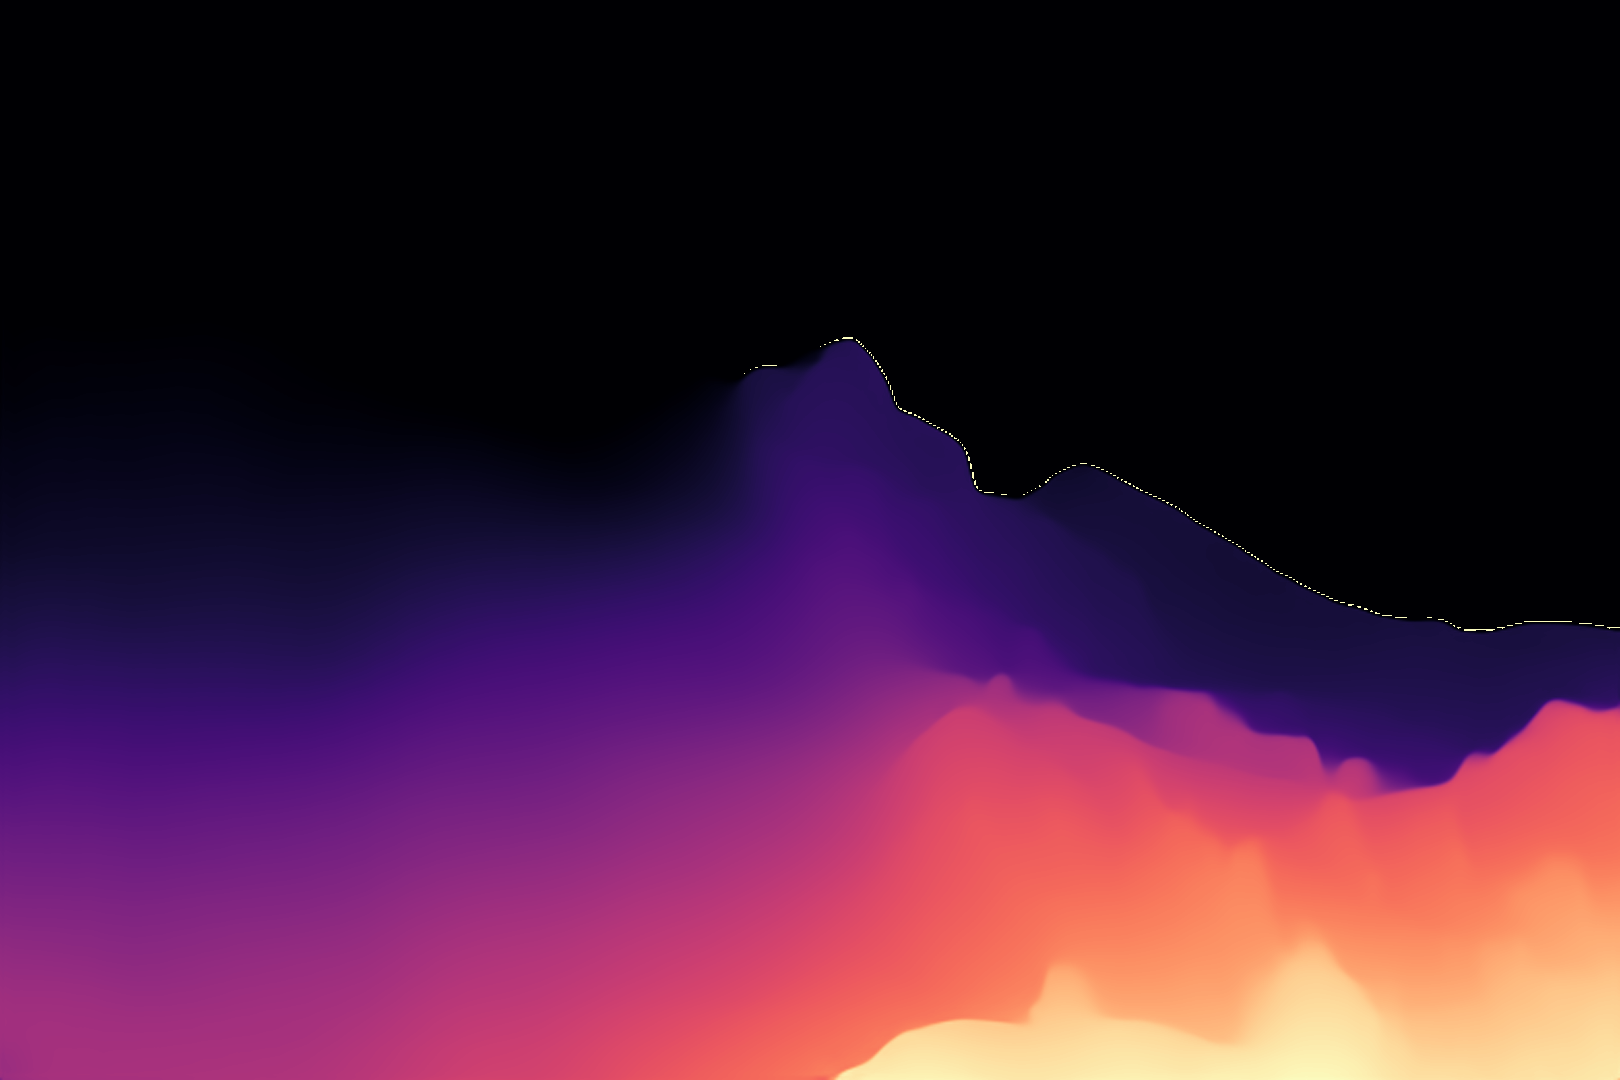
\includegraphics[width=0.32\textwidth]{./figures/luhinterland_v1-small.png}
        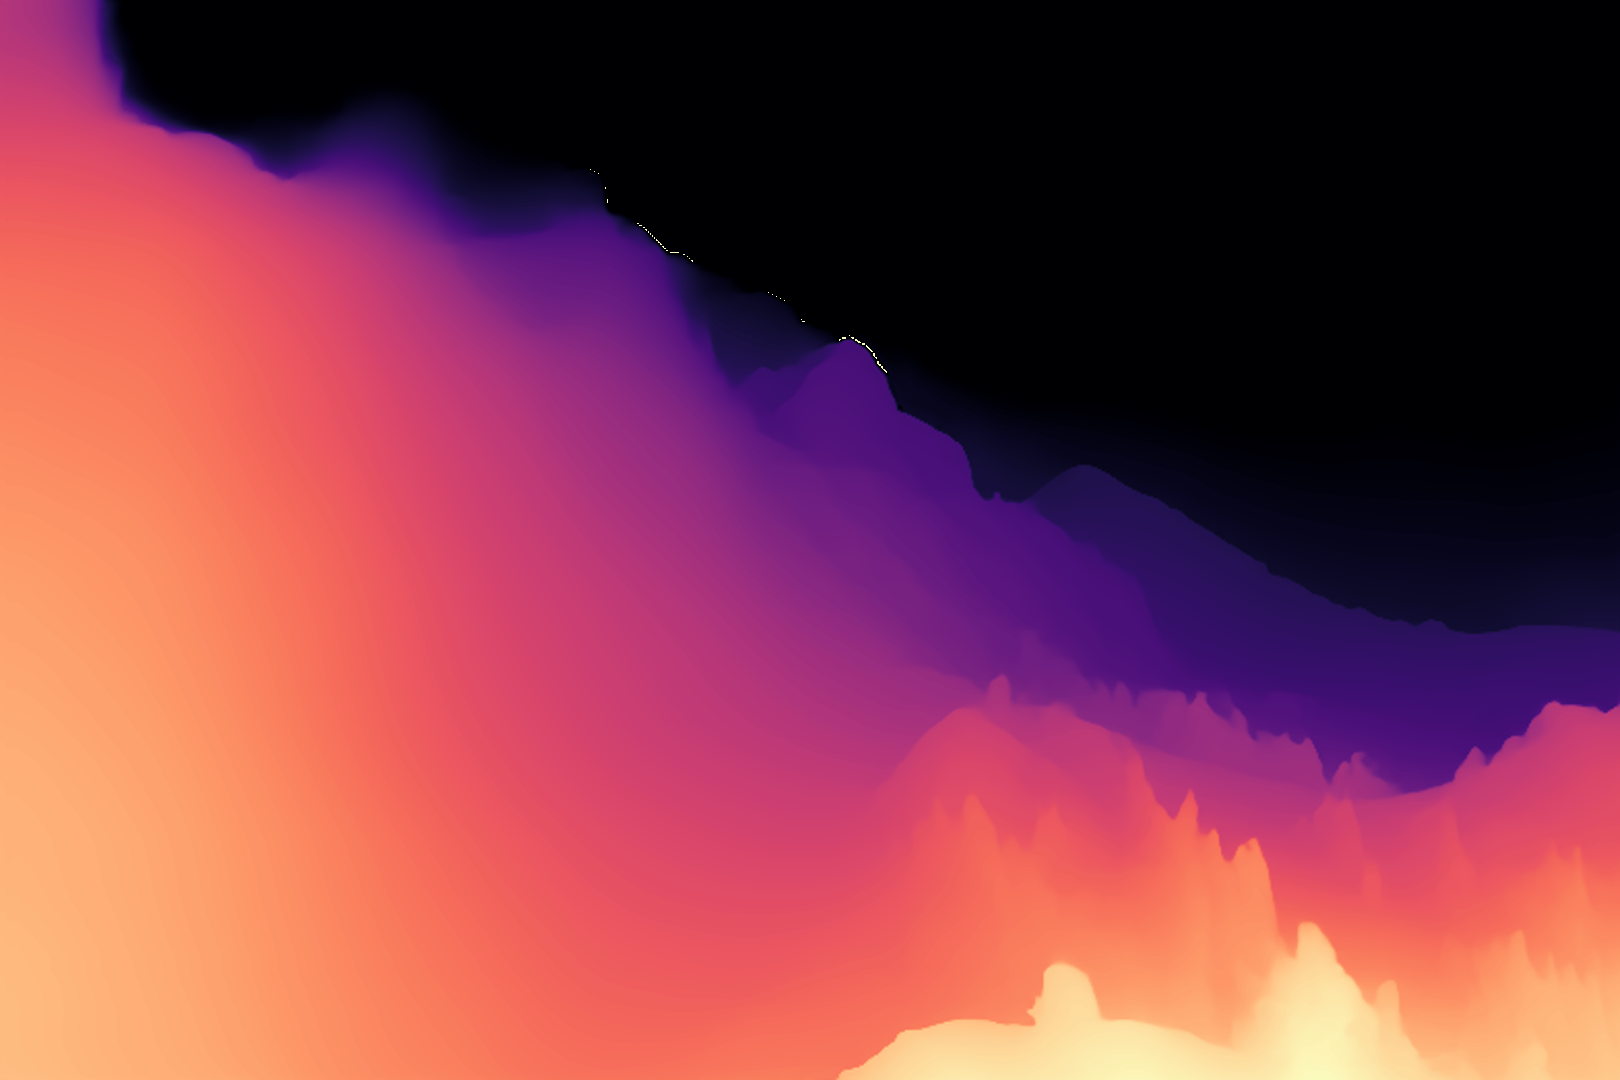
\includegraphics[width=0.32\textwidth]{./figures/luhinterland_v2-small.png}
        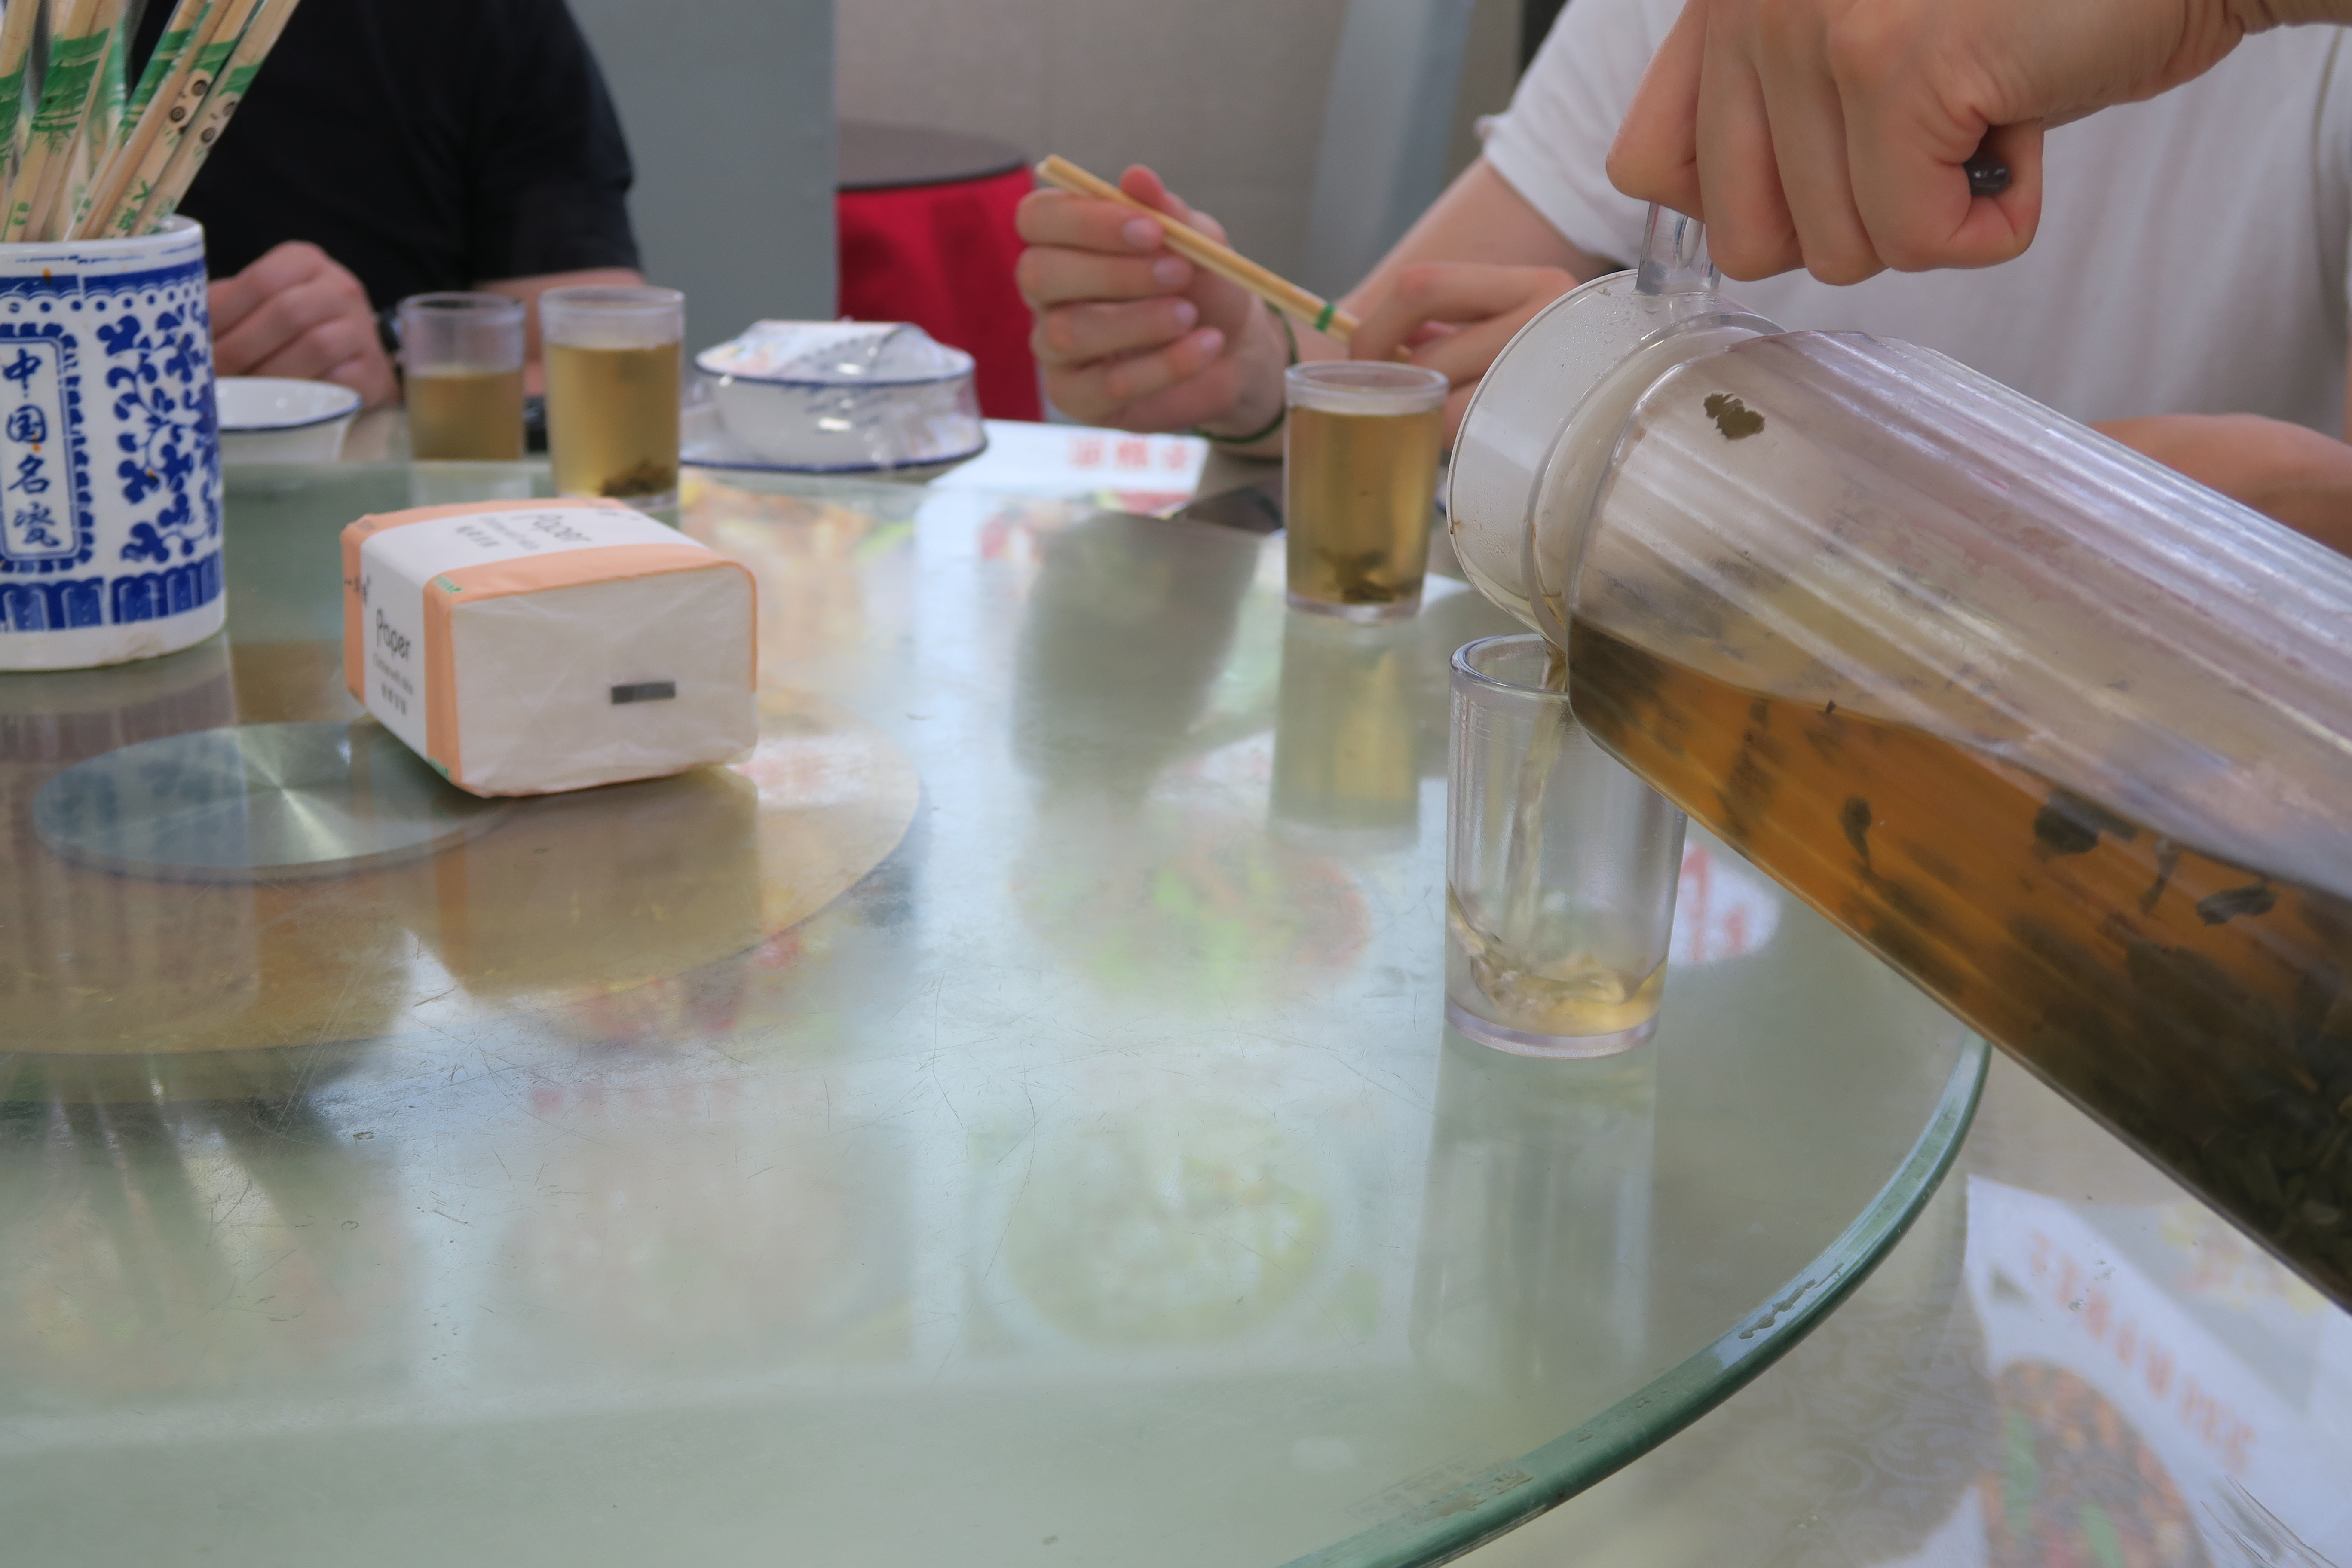
\includegraphics[width=0.32\textwidth]{./figures/tea.JPG}
        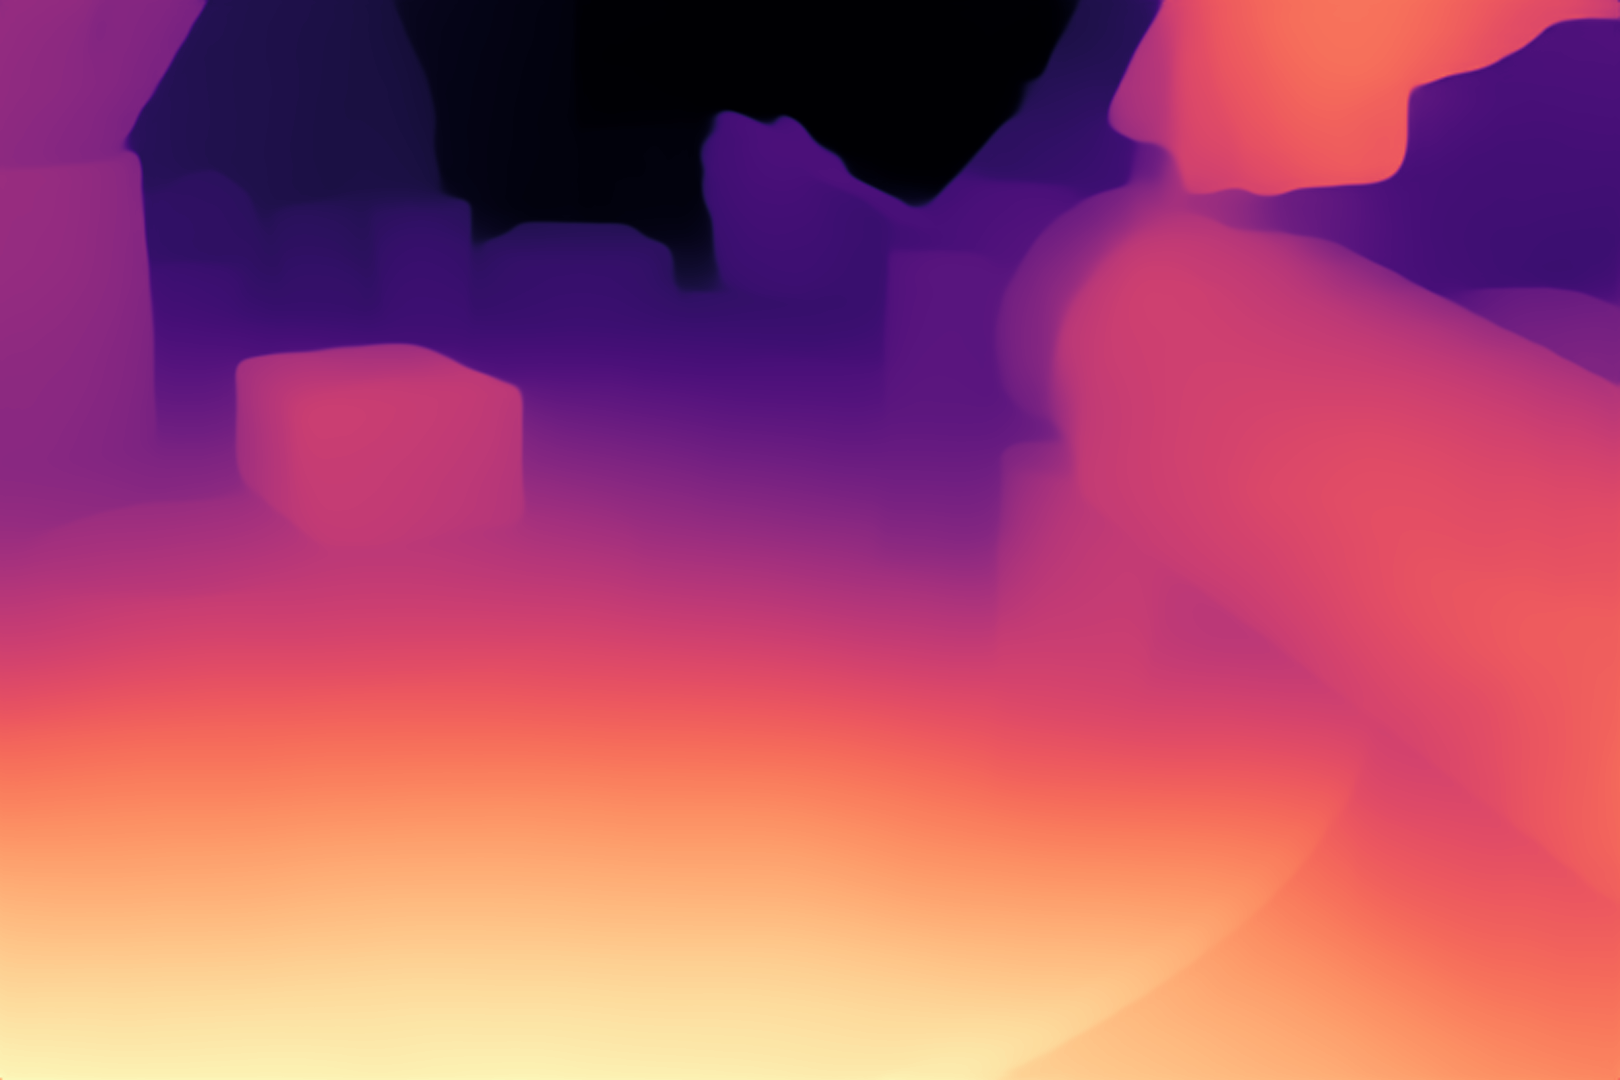
\includegraphics[width=0.32\textwidth]{./figures/tea_v1-small.png}
        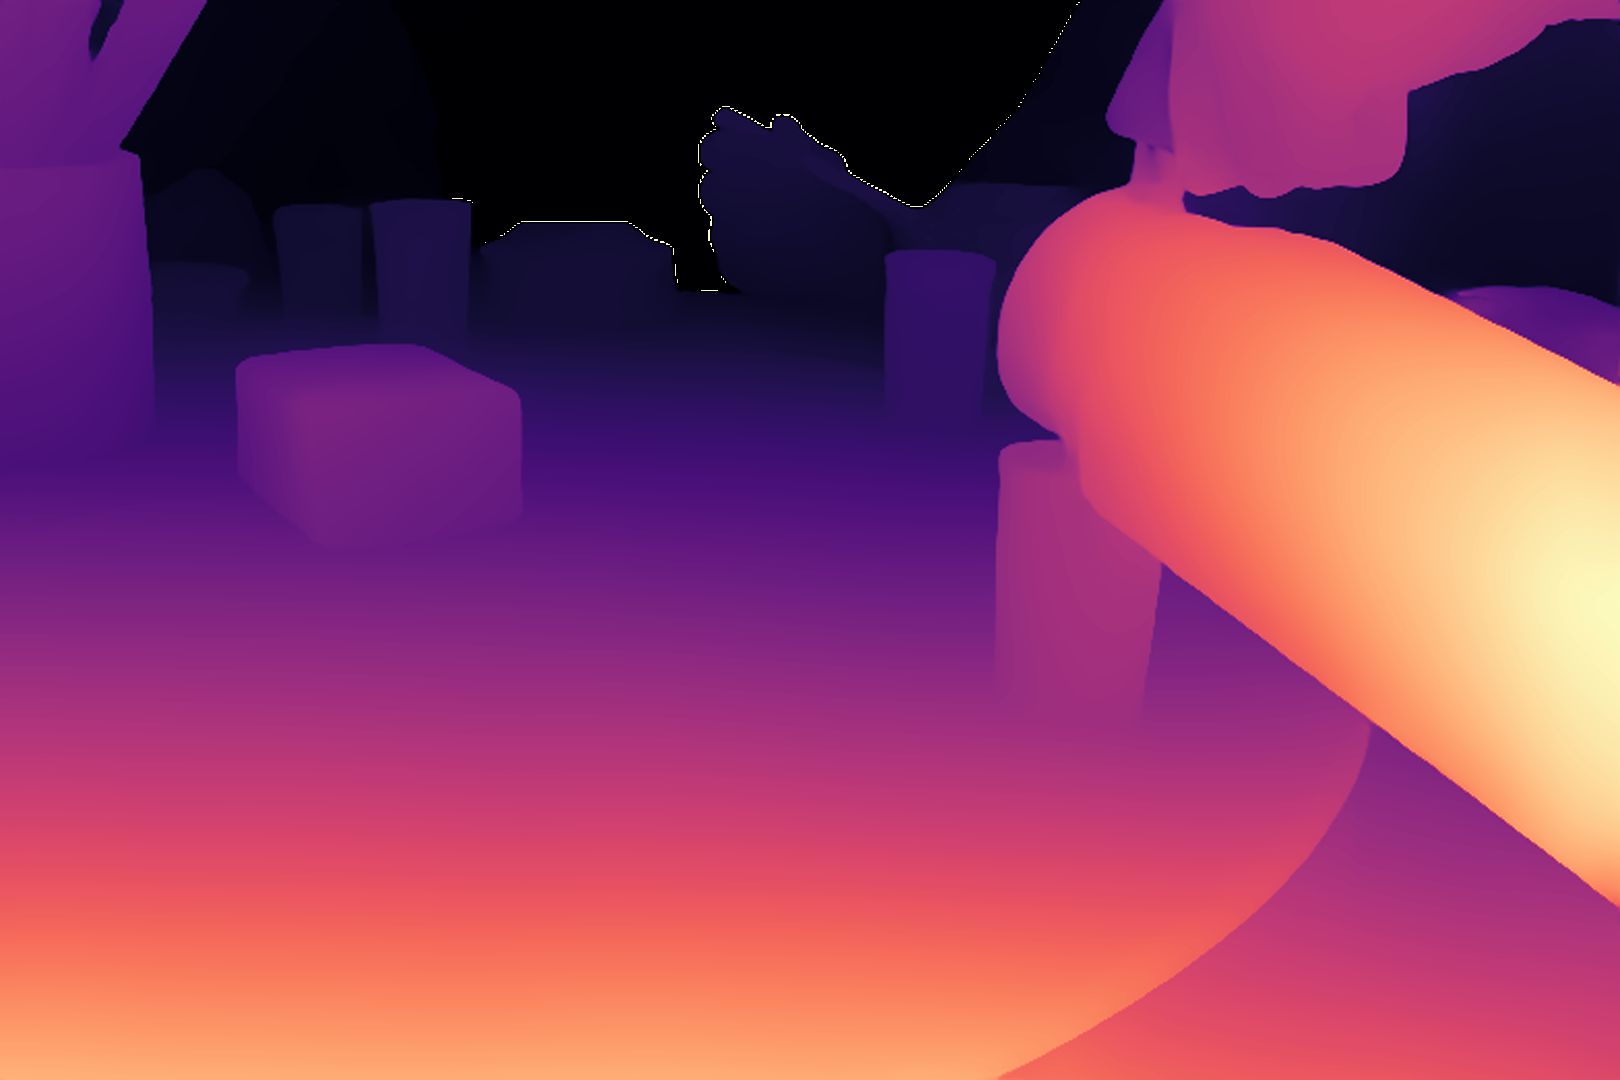
\includegraphics[width=0.32\textwidth]{./figures/tea_v2-small.png}
        \caption{Original (left), V1 (middle), and V2 (right) depth map}
        \label{fig:res_2}
    \end{figure}
\end{frame}

\begin{frame}
    \frametitle{Live Demo}
    
\end{frame}

% graphical overview
\begin{frame}
    \frametitle{Summary}
    
        
    \begin{figure}
        \centering
        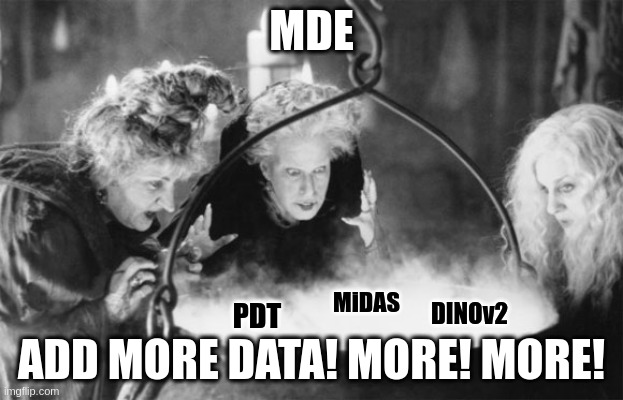
\includegraphics[width=0.49\textwidth]{./figures/summary_v1.jpg}
        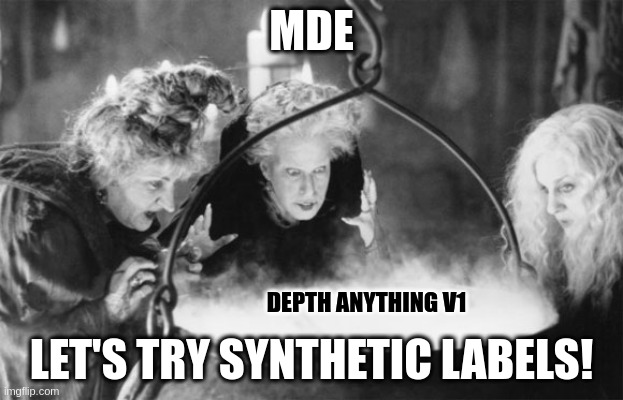
\includegraphics[width=0.49\textwidth]{./figures/summary_v2.jpeg}
        \caption{Summary of Depth Anything V1 (left) and V2 (right).}
        \label{fig:summary}
    \end{figure}
\end{frame}


\begin{frame}
    \frametitle{Sources}
    \scriptsize
    
    \textbf{Presentation \& Code} \href{https://github.com/birawaich/thu_mavi_paperpresentation}{Github}\footnote{ \tiny For print: \url{github.com/birawaich/thu_mavi_paperpresentation}}
    
    \textbf{Papers}
    \begin{itemize}
        \item \href{https://arxiv.org/abs/2401.10891}{Depth Anything: Unleashing the Power of Large-Scale Unlabeled Data}
        \item \href{https://arxiv.org/abs/2406.09414}{Depth Anything V2}
        \item \href{https://arxiv.org/abs/1907.01341}{MiDaS}
        \item \href{https://arxiv.org/abs/2304.07193}{DINOv2}
        \item \href{https://arxiv.org/abs/1905.04899}{CutMix}
        \item \href{https://arxiv.org/abs/2302.12288}{ZoeDepth}
        \item \href{https://arxiv.org/abs/2312.02145}{Marigold}
    \end{itemize}
    
    \textbf{Pictures}
    if not noted differently, captured myself
    
    \textbf{Illustrations}
    if not noted differently, created myself
    
    
\end{frame}


\begin{frame}
    \frametitle{Backup Slides}
    \scriptsize
    
    \textbf{MiDaS}
    \begin{itemize}
        \item = Mixing Datasets for Zero-shot Cross-dataset Transfer $\leadsto$ enables training cross datasets!
        \item 2024; Intel, ETHZ
        \item affine-invariant Loss $\mathcal{L}_\text{ssi}$
        \item gradient matching Loss $\mathcal{L}_\text{gm}$
    \end{itemize}

    \textbf{DINOv2}
    \begin{itemize}
        \item 2024; Meta AI
        \item = variety of pretrained visual models running on ViT architectures
        \item extract features that can be broadly used
    \end{itemize}

    \textbf{DPT}
    \begin{itemize}
        \item = Dense Periodic Transformer
        \item 2021; Intel
        \item Idea: Vision Transformer (ViT) instead of Fully-Convolution Network for dense predicitons e.g. Molecular Depth Estimation
    \end{itemize}

    
\end{frame}
\begin{frame}
    \scriptsize
    \textbf{Marigold}
    \begin{itemize}
        \item 2024; ETHZ
        \item MDE going the route of Stable Diffusion
        \item based on text-to-image diffusion model
        \item can do fine details well $\leadsto$ Deep Anything V2 Goals
    \end{itemize}
    \textbf{ZoeDepth}
    \begin{itemize}
        \item = Zero-shot Transfer by Combining Relative and Metric Depth
        \item 2023; KAUST, Intel
        \item does not focus on only relative depth, but also metric!
        \item $\rightarrow$ used in V1 to also do Metric Depth Estimation by swapping the Encoder and retaining the ZoeDepth Architecture
    \end{itemize}
\end{frame}
\begin{frame}        
    \textbf{Quantitative Results V1}
    \begin{figure}
        \centering
        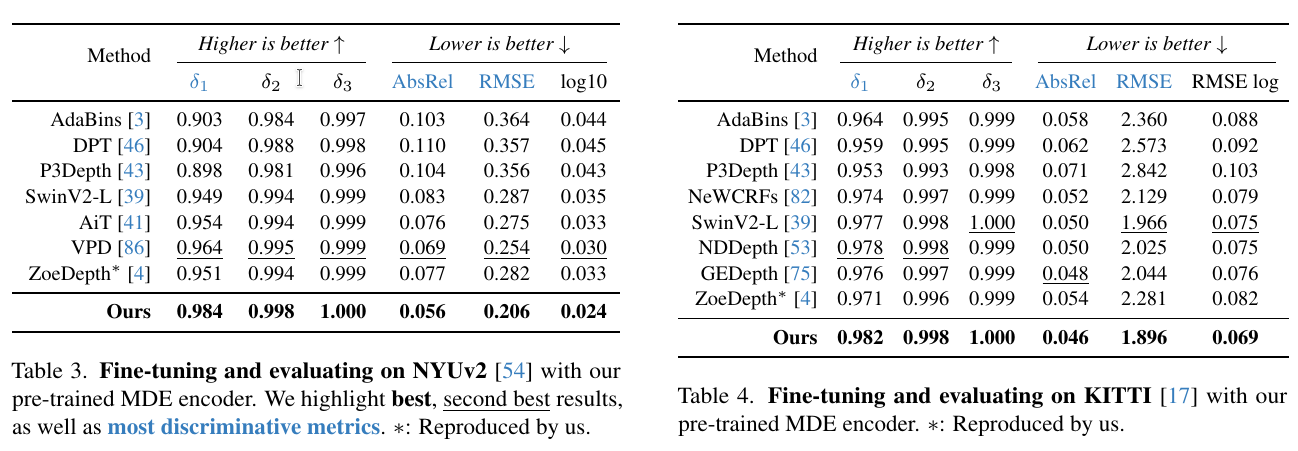
\includegraphics[width=\textwidth]{./figures/screenshot_table-results_v1.png}
        \caption{Quantitative Results of V1 from the paper}
        \label{fig:res_quant_v1}
    \end{figure}
\end{frame}
\begin{frame}
    \scriptsize
    \textbf{DA-2K Benchmark}
    \begin{itemize}
        \item Benchmark proposed by authors of Deep Anything V2
        \item Reasons
        \begin{itemize}
            \item Limited Diversity
            \item Low Resolution
            \item Noisy Labels
        \end{itemize}
        \item Implementation
        \begin{itemize}
            \item Use \underline{Expert Models} which provide "ground truth" between pixel pairs
            \item In case of no agreement $\rightarrow$ human
        \end{itemize}
    \end{itemize}
\end{frame}
\begin{frame}        
    \textbf{Quantitative Results V2}
    \begin{figure}
        \centering
        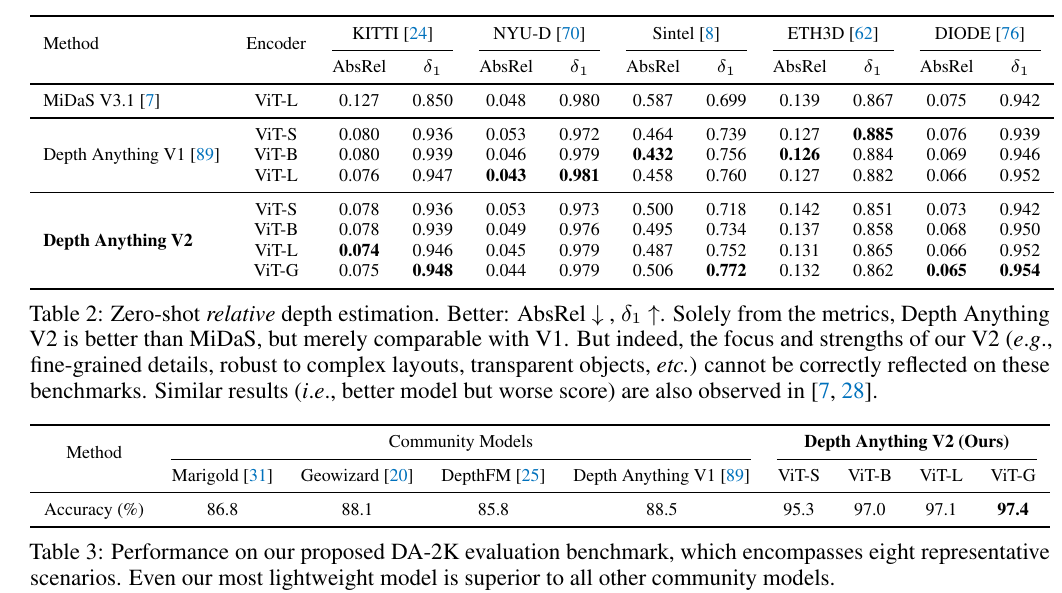
\includegraphics[width=\textwidth]{./figures/screenshot_table-results_v2.png}
        \caption{Quantitative Results of V2 from the paper}
        \label{fig:res_quant_v2}
    \end{figure}
\end{frame}
    

\end{document}
